\clearpage
\appendix
\counterwithin{equation}{section}
\renewcommand{\theequation}{\thesection.\arabic{equation}}

\section{Proofs}
\label{app:proofs}

\subsection{Count law and conditional information}
\label{app:model}

The probability generating function of one negative binomial offspring count is $[1+(R_t/k)(1-z)]^{-k}$. Conditional independence raises this function to the power $n$, and substituting $z\mapsto1-\rho+\rho z$ for independent reporting gives $[1+(\rho R_t/k)(1-z)]^{-nk}$, which proves Eq.~\eqref{eq:observed}; its derivatives give the stated moments.

For fixed, known $(n,\rho,k)$ and $R>0$, the count likelihood has the score and Fisher information:
\begin{equation}
 \dot\ell(R)=\frac{c}{R}-\frac{(c+nk)\rho}{k+\rho R}
 =\mathcal I(R)(\Rhat-R),\qquad
 \mathcal I(R)=\frac{m}{R+\rho R^2/k}.
 \label{eq:score}
\end{equation}
By Eq.~\eqref{eq:score}, $\Var(\Rhat\mid R)=\mathcal I(R)^{-1}$. The support does not depend on $R$, so the regular one-parameter Cram\'er--Rao inequality applies to estimators unbiased for every $R$ and gives the attained bound stated in Section~\ref{sec:model-targets} \citep{lehmann1998theory}. The bound therefore applies to estimators unbiased for every $R$ with $\rho$ and $k$ known; biased estimators and unknown nuisance parameters require a separate analysis.

\subsection{Proof of Proposition~\ref{prop:average}}
\label{app:prop1}

Let $e_t=\Rhat_t-R_t$. The error is conditionally centred, $\E(e_t\mid R_t)=0$, and its second moments are as follows:
\begin{equation}
 \E(e_t^2)=\frac{\E R_t+\rho\E R_t^2/k}{m}=\frac{A}{m},
 \qquad \E[e_t(R_t-\Rbar)]=0.
\end{equation}
Squaring Eq.~\eqref{eq:error-split} proves Eq.~\eqref{eq:var-average}. Any estimator based on the same count and unbiased conditional on every $R_t$ has expected conditional variance at least $\E[\mathcal I(R_t)^{-1}]=A/m$, and its process-mean risk adds the same $v_R$. At fixed $\rho$, $k$ and transmission law, $[V(m)-V(2m)]/V(m)=1/[2(1+m/\mx)]$ for $v_R>0$. The comparison changes exposure $n$; it does not hold unchanged when the reporting probability changes. The shrinkage weight in Eq.~\eqref{eq:shrink-weight} is $\Cov(R_t,\Rhat_t)/\Var(\Rhat_t)=v_R/V(m)$.

\subsection{Proof of Corollary~\ref{cor:targets}}
\label{app:cor-targets}

Conditional on the path $R_{1:T}$, the $e_t$ are independent and centred, hence pairwise uncorrelated and orthogonal to every square-integrable function of the path. Thus the average of $e_1,\dots,e_T$ has second moment $A/(Tm)$, and $\Var(\overline{\Rhat}_T)=\Var(\Rbar_T)+A/(Tm)$. Under the stated stationary autocovariance, summing all covariance pairs gives $T^2\Var(\Rbar_T)=v_RS(\phi,T)$ with the first expression in Eq.~\eqref{eq:ar-sum}, and the finite geometric sum yields the second \citep{hamilton1994time}. Summing spatial covariance pairs in the same way gives Eq.~\eqref{eq:pooling}, for any admissible correlation matrix.

\subsection{Proof of Proposition~\ref{prop:report-noise} and Corollary~\ref{cor:report-current}}
\label{app:prop2}

Write $z_t=p_t/\rho$ and $u_t=C_t/m-z_tR_t$. Conditional on $(R_t,p_t)$, $u_t$ has zero mean. Independence of $p_t$ and $R_t$, with $\E z_t=1$ and $\E z_t^2=1+\tau^2$, gives:
\begin{equation}
 \E(u_t^2)=\frac{\Rbar+\rho(1+\tau^2)(\Rbar^2+v_R)/k}{m}=\frac{A_H}{m}.
\end{equation}
The error $\Rhat_t-R_t=u_t+(z_t-1)R_t$ has uncorrelated terms, and the second has expected square $\tau^2(\Rbar^2+v_R)=v_H$, which proves Eq.~\eqref{eq:vH-current}. Because $\E(\Rhat_t-R_t\mid R_t)=0$, process-mean risk adds $v_R$. Under the additional cross-period assumptions of Corollary~\ref{cor:report-current}, the errors are centred and independent given the transmission path after integrating out reporting, which gives Eq.~\eqref{eq:report-means}.

For the identification statement, set $U=(1+\tau^2)(\Rbar^2+v_R)$. The two moments of the scaled count are:
\begin{equation}
 \E\Rhat_t=\Rbar,\qquad
 \Var(\Rhat_t)=U-\Rbar^2+\frac{\Rbar+\rho U/k}{m}.
 \label{eq:moment-identification}
\end{equation}
Whenever distinct admissible values of $\tau^2$ give $v_R=U/(1+\tau^2)-\Rbar^2\ge0$, the moments in Eq.~\eqref{eq:moment-identification} coincide, and varying an exogenous $m$ does not separate them. This proves nonidentification by these moments only; it does not assert equality of full count distributions.

For $v_R>0$, the crossover scale with volatile reporting, $m_{\times,H}=A_H/(v_R+v_H)$, satisfies:
\begin{equation}
 \mx-m_{\times,H}
 =\frac{\tau^2(\Rbar^2+v_R)\Rbar(1+\rho\Rbar/k)}{v_R(v_R+v_H)}\ge0.
 \label{eq:mx-gap}
\end{equation}
Equality holds exactly when $\tau=0$.

\subsection{Observed denominator}
\label{app:observed-denominator}

Let $M_t\sim\Bin(n,\rho)$ be independent of the offspring given $n$, and write $M_t=m(1+u_t)$, so that $\E u_t=0$ and $\Var(u_t)=(1-\rho)/m$. Then $\tilde R_t=\Rhat_t/(1+u_t)$. To first order in $u_t$ and $\Rhat_t-R_t$, the error is approximately:
\begin{equation}
 \tilde R_t-R_t\approx(\Rhat_t-R_t)-R_tu_t .
\end{equation}
Given $(n,R_t)$, $u_t$ is independent of $\Rhat_t-R_t$ and centred, so the cross term vanishes and
$\E[(\tilde R_t-R_t)^2]\approx A/m+(1-\rho)\E(R_t^2)/m$, which is Eq.~\eqref{eq:observed-denominator}. The Monte Carlo check in Table~\ref{tab:ma_targets_observed} draws $R_t$ from a gamma law with the stated moments and would discard draws with $M_t=0$, none of which occurred at the scales shown. The approximation neglects the convexity of $1/(1+u_t)$, which inflates the error when $m$ is small; at $m=10$ the Monte Carlo error is 1.64 times the delta value.

\subsection{Reporting shocks in the ratio statistic}
\label{app:ratio-shocks}

Let the count of week $t$ in a state be reported with probability $\rho z_t$, where the shocks $z_t$ are independent between weeks with $\log z_t\sim N(-s^2/2,s^2)$. To first order, the statistic in Eq.~\eqref{eq:ra} satisfies $\log R_{A,t}\approx\mathrm{const}+\kappa(g)\log g_t$ with $\kappa(g)=(g_\mu/7)/[1+\theta\log(g)/7]$, because $\alpha\theta=g_\mu$. The shocks enter the observed growth factor as $\log g_t=\log g^{\mathrm{tr}}_t+\eta_t$, with $\eta_t=\log z_{t+1}-\log z_t$ and $g^{\mathrm{tr}}_t$ the growth factor without shocks. Hence $\Var(\eta_t)=2s^2$, and the relative variance that the shocks add to the ratio statistic is:
\begin{equation}
 \tilde v_H\approx2\kappa^2s^2 .
 \label{eq:ratio-shock}
\end{equation}
This component does not scale with count and therefore enters the intercept $a$. A reporting level that is constant over consecutive weeks of a state ($z_{t+1}=z_t$) gives $\eta_t=0$ and cancels. Consecutive rows share one shock with opposite signs, so $\Cov(\eta_t,\eta_{t+1})=-s^2$ and their correlation is $-1/2$. The affine fit uses squared deviations, and for jointly Gaussian terms a correlation of $-1/2$ becomes a correlation of $+1/4$ between their squares. Resampling single weeks does not preserve this serial dependence, so interval coverage was checked directly. Under the audit generators S6 and S8 (Appendix~\ref{app:audit}), which contain such shocks, the pigeonhole bootstrap intervals for $a$, $b$ and $b/a$ covered the Monte Carlo means of their estimators in at least 99.5\% of 400 panels (Table~\ref{tab:ma_coverage}). Under the fresh-draw generators with such shocks its standard deviation for $a$ exceeded the Monte Carlo value by a factor of 1.55--1.67 (Table~\ref{tab:r2-bootstrap-sd}). For the realised mean over $T$ consecutive rows of one state the mean of the shock terms telescopes to $(\log z_{T+1}-\log z_1)/T$, so their contribution to the error of the realised mean falls as $T^{-2}$ rather than $T^{-1}$. With $\kappa$ near 0.5 for the primary interval and $s=0.122$ as in generator S6, Eq.~\eqref{eq:ratio-shock} gives a shock component of about half the observed intercept.

\section{Extensions}
\label{app:extensions}

\subsection{Forecasting and shrinkage}
\label{app:forecast}

Under fixed, known reporting and the stationary covariance of Corollary~\ref{cor:targets}, with the counting error at $t$ centred given the transmission path, the best forecast of $R_{t+1}$ of the form $\Rbar+\lambda(\Rhat_t-\Rbar)$ has the weight and risk:
\begin{equation}
 \lambda^*=\frac{\phi v_R}{v_R+A/m}=\phi\,\gamma(m),\qquad
 \mathrm{MSE}_{\mathrm{lin}}=v_R-\frac{\phi^2v_R^2}{v_R+A/m}.
 \label{eq:forecast}
\end{equation}
This follows from $\Cov(\Rhat_t,R_{t+1})=\phi v_R$. The forecast weight in Eq.~\eqref{eq:forecast} is the shrinkage weight discounted by persistence, and its limit risk is $(1-\phi^2)v_R$. For the process mean, shrinking $\Rhat_t$ towards a fixed benchmark $\mu_0$ with oracle weight $V(m)/[V(m)+(\mu_0-\Rbar)^2]$ can give risk below $v_R$; this lies outside the conditionally unbiased class of Proposition~\ref{prop:average}, and estimating the weight requires its own risk analysis.

\subsection{Allocation between periods, cases and coverage}
\label{app:allocation}

\begin{proposition}[Budget allocation between periods and cases]
\label{prop:allocation}
Under H1--H4, independent, identically distributed transmission periods, conditionally independent counts, fixed $\rho$ and linear costs, let the budget be $\mathcal B=T(c_0+c_1m)$ with $c_0,c_1>0$, and treat $T\ge1$ and $m>0$ as continuous. If $v_R>0$ and $\mathcal B>c_0$, process-mean risk $(c_0+c_1m)(v_R+A/m)/\mathcal B$ is strictly convex in $m$ and is minimised at:
\begin{equation}
 m^*=\min\{(c_0\mx/c_1)^{1/2},\ (\mathcal B-c_0)/c_1\}.
 \label{eq:optimal-m}
\end{equation}
\end{proposition}

The optimum in Eq.~\eqref{eq:optimal-m} has the form of cluster-size allocation in survey sampling and multilevel design \citep{cochran1977sampling, raudenbush1997statistical}: cases per period should grow only with the square root of $\mx$ and of the relative cost of a period. Integer designs compare the risk over feasible integer $T$ with $n_T=\lfloor(\mathcal B/T-c_0)/(c_1\rho)\rfloor$. Under temporal dependence the variance term becomes $v_RS(\phi,T)/T^2$ and no closed-form optimum follows.

\begin{corollary}[Coverage against completeness]
\label{cor:switch}
Under H2--H5, let $p_t$ be the participating fraction of $\nu$ independent reporting units, each participating with probability $\rho$, so that $\tau^2=(1-\rho)/(\rho\nu)$. A proportional increase in completeness $\rho$ reduces single-period process-mean risk more than the same proportional increase in exposure $n$ exactly when $m>\rho^2(\nu-1)/k$.
\end{corollary}

Write the single-period risk as $v_R+v_H+A_H/m$ with $v_H=\tau^2Q$, $Q=\Rbar^2+v_R$ and $m=\rho n$, and differentiate with respect to $\log\rho$ and $\log n$. The difference of the two derivatives is:
\begin{equation}
 \frac{\partial\,\mathrm{risk}}{\partial\log\rho}-\frac{\partial\,\mathrm{risk}}{\partial\log n}
 =-\frac{Q}{kn}\left[\frac{kn+\rho}{\rho\nu}-1\right].
\end{equation}
Because $Q/(kn)>0$, the difference is negative, and a proportional increase in $\rho$ lowers the risk more than the same increase in $n$, exactly when $kn+\rho>\rho\nu$, that is, when $m>\rho^2(\nu-1)/k$. The mechanism is assumed; observed facility participation alone does not imply it.

\subsection{Number of seasons}
\label{app:seasons}

Suppose $S\ge2$ season effects are independent Gaussian with unknown mean and variance $v_S>0$, and the count law given the effects does not depend on these parameters. Any estimator unbiased for $v_S$ then has relative standard error at least $(2/(S-1))^{1/2}$. Observing the effects themselves gives at least as much information as the counts, and their sample variance is the minimum-variance unbiased estimator \citep{lehmann1998theory, searle1992variance}. With the four seasons analysed here the bound is $(2/3)^{1/2}=0.82$, and additional admissions within the same seasons leave it unchanged. This bound concerns the precision with which the between-season variance component can be estimated; it is distinct from the power of a test of equal season intercepts, which depends on the size of the season differences relative to their standard errors and is reported in Section~\ref{sec:res-season}.

\subsection{Thinning and the delta approximation}
\label{app:thinning-exact}

Binomial thinning provides a further check on the counting slope. Each unique state-week count is thinned once to $\Bin(C,q)$ for $q\in\{0.8,0.6,0.5,0.4,0.3,0.2,0.1\}$, and the thinned value is reused in every ratio that contains it. Recomputing the statistic and the fit, with the original $C_t$ as regressor, gives the thinning response:
\begin{equation}
b(q)-b(1)\simeq c\,(1/q-1).
\label{eq:thinning}
\end{equation}
Under the delta approximation $c=\bP$ whatever the original counting variation, because thinning adds known binomial variance. The ratio $c/\bP$ is therefore a check of that approximation and not of the data-generating process. Because the check of Eq.~\eqref{eq:thinning} rests on a delta approximation, its exact expectation was computed on the observed counts. For each retention probability $q$ the expected increment of the inverse-count slope was evaluated by summing over the binomial law of every thinned count (Table~\ref{tab:ma_thinning_exact}; Fig.~\ref{fig:thinning-exact}A). The exact increment rate is 0.467 at $q=0.8$, rises to 0.505 at $q=0.3$ and falls to 0.480 at $q=0.2$ and 0.384 at $q=0.1$. The least-squares rate over all $q$ is 0.408, or 0.917 $\bP$, against the Monte Carlo estimate 0.405 (0.366--0.441), or 0.909 (0.810--0.999) $\bP$ (Table~\ref{tab:thinning}).

The pooled rate is dominated by the smallest retention probability. The value $q=0.1$ carries 76\% of the leverage in the least-squares rate (Fig.~\ref{fig:thinning-exact}B), and without it the rate is 0.488, or 1.096 $\bP$. At $q=0.1$ many thinned counts are small, and the delta approximation of the variance of a log thinned count fails there. At $C=5$ and $q=0.1$ the exact added variance of $\log(\Bin(C,q)+0.5)$ is 0.21 of the delta value (Table~\ref{tab:ma_varlog}; Fig.~\ref{fig:thinning-exact}C). The positive-part truncation of the fitted mean never binds. The shortfall of the pooled rate below $\bP$ is therefore a property of the approximation at small thinned counts, not evidence about the data-generating process.

In the audit the ratio $c/\bP$ lies in 0.95--1.00 under S0, 0.96--1.04 under S4, 0.87--0.98 under S5, 0.83--0.93 under S3 and 0.81--0.92 under S6. The observed value lies outside the ranges of the generators with Poisson offspring (S0, S1, S2P and S4) and inside those with negative binomial offspring, but its confidence interval overlaps all of them. Because thinning adds known binomial variance whatever the original counting process, the check cannot separate offspring overdispersion from under-reporting.

\section{Known-truth simulation audit}
\label{app:audit}

\subsection{Design}
\label{app:audit-design}

The audit is a simulation study with known truth, reported under the aims, data-generating mechanisms, estimands, methods and performance measures structure of \citet{morris2019using}. It asks what $a$, $b$, $b/a$ and the thinning rate recover on the sampling design of the application. Synthetic counts were generated on the exact $R_A$ design: the 1,748 rows, 1,969 unique state-weeks and 210 state runs of the data. Each run is simulated as a whole with shared counts, so that one week's count is the next week's denominator. The expected count is carried forward by the true growth factors, and the geometric-mean observed growth $g_0=1.407$ is used for transitions that are not scored. The simulated $C_t$ serves as the count scale, the filter $C_t\ge5$ is re-applied, and the estimand of each row is the transform~\eqref{eq:ra} of its true growth factor.

Two alignment steps fix the level of the synthetic panels, and the quantities they fix are calibration targets rather than tests. Each run is level-anchored to the geometric mean of its observed counts, and one scale factor per generator, between 0.797 and 0.844, sets the Monte Carlo mean of the median retained count to the observed median of 45. In every generator with transmission heterogeneity, the amplitude of that heterogeneity is then set so that the Monte Carlo mean of the fitted intercept equals the observed $a$. The slope ratio $b/\bP$, the crossover $b/a$, the thinning rate, the pooled-to-within-state slope ratio, the reduction of $a$ under week centring and the score contrast between affine and power-law fits are not targeted and serve as tests. A generator passes a test when the observed point value lies inside its 2.5--97.5\% Monte Carlo range. This decision rule and the week-centring test were fixed after the generators had first been compared with the data, and Table~\ref{tab:ma_tests} applies them to every generator. The lower tail of the retained counts matches the data (10th percentiles 10--11 against 10), but the upper tail does not, since the generators' 90th percentiles are 263--324 against 389 observed (Table~\ref{tab:ma_audit_loss}). Post-stratifying retained rows to the observed deciles of the count moves intercept recovery by at most 3.2\%.

Table~\ref{tab:ademp} sets out the design. The generators span the mechanisms that the diagnostics are meant to separate, from independent Poisson counts (S0) to scale-dependent heterogeneity combined with state-week reporting shocks (S8). Generator S9, which carries half of the S8 transmission heterogeneity in a national calendar-week component, was added after the others had been compared with the data. All generators in this appendix keep one heterogeneity field fixed across replicates; the interval checks of the analysis plan (Section~\ref{sec:res-validity}) redraw it in every replicate.

\begin{table}[!tbp]
\centering
\small
\caption{Design of the known-truth audit}
\label{tab:ademp}
\begin{tabularx}{\linewidth}{@{}>{\raggedright\arraybackslash}p{0.2\linewidth}>{\raggedright\arraybackslash}X@{}}
\toprule
Element & Specification \\
\midrule
Aim & What $a$, $b$, $b/a$, $b/\bP$ and the thinning rate $c$ recover on the $R_A$ design of the application \\
Estimands & Transmission relative variance $\tilde v_R$; total $\tilde v_R+\tilde v_H$ when reporting shocks are present; expected slope relative to $\bP$ \\
Methods & The pipeline of the application: $R_A$ transform, relative squared deviation, gamma FGLS affine fit, plug-in $\bP$, within-state slope, week centring, score contrast between power-law and affine fits (positive values favour the affine form) \\
Performance measures & Monte Carlo mean with its standard error; 2.5\% and 97.5\% Monte Carlo limits; ratio of means for recovery; quantile of the observed value among simulated values; interval coverage \\
Calibration targets & Median retained count (all generators); mean fitted intercept equal to the observed $a$ (generators with heterogeneity) \\
Tests & $b/\bP$, $b/a$, thinning rate, ratio of pooled to within-state slope, week-centring reduction of $a$, score contrast; a test is passed when the observed value lies inside the 2.5--97.5\% Monte Carlo range \\
Replicates & 200 panels per generator; five streams of 200 for score-contrast quantiles; thinning 100 panels with 20 draws per level; coverage 400 panels per generator (S1, S6, S8, S9) with 200 bootstrap draws each; held-out reference 200 panels per generator \\
\midrule
\multicolumn{2}{@{}l}{\textit{Data-generating mechanisms}} \\
S0 & Constant growth $g_0$, independent Poisson counts \\
S1 & Independent lognormal growth factors ($\sigma=0.247$), Poisson counts \\
S2 & Constant growth, negative binomial offspring ($k=0.3$), binomial reporting at $\rho=0.25$ \\
S2P & S2 with Poisson offspring (pure branching chain with reporting) \\
S3 & S1 combined with the S2 counting model \\
S4 & Growth heterogeneity split equally between state and national-week components, Poisson counts \\
S5 & S4 combined with the S2 counting model \\
S6 & S3 with a state-week reporting shock $\rho_{st}=0.25z_{st}$, $\log z_{st}\sim N(-s^2/2,s^2)$, $s=0.122$ \\
S7a, S7b & S3 with heterogeneity $\sigma^2(\mu)=\sigma_0^2(\mu/45)^{-\gamma}$ for expected count $\mu$, $\gamma=0.25$ and $0.5$ \\
S8 & S3 with scale-dependent heterogeneity ($\gamma=0.25$) and state-week reporting shocks ($s=0.133$) \\
S9 & S8 with half of the transmission heterogeneity carried by the national-week component of S4 ($s=0.132$) \\
\bottomrule
\end{tabularx}
\par\smallskip
\begin{minipage}{\linewidth}\footnotesize\raggedright
In S6, S8 and S9 the shock scale is chosen so that transmission and the shock each carry about half of the variance target set by the observed $a$. Tests are statistics that no alignment step targets.
\end{minipage}
\end{table}

\subsection{Results}
\label{app:audit-results}

Without reporting shocks the intercept tracks the relative variance of transmission. When transmission is constant (S0, S2 and S2P) the fitted intercept is essentially zero. With independent heterogeneity, the ratio of $a$ to the true relative variance on the retained rows is 1.01 (Monte Carlo range 0.93--1.09) under S1 and 1.02 (0.91--1.13) under S3. With structured heterogeneity it is 1.12 (1.04--1.19) under S4 and 1.15 (1.06--1.27) under S5 (Table~\ref{tab:ma_audit_loss}; Fig.~\ref{fig:audit}C). With reporting shocks that are fixed across replicates the intercept approximates the sum of both components: under S6, $a$ is 1.01 (0.87--1.14) times the total $\tilde v_R+\tilde v_H$ and 2.02 (1.71--2.29) times $\tilde v_R$ alone. Scale-dependent heterogeneity biases the intercept in the other direction, to 0.68 (0.60--0.78) and 0.43 (0.37--0.50) of the true relative variance under S7a and S7b, because variation that shrinks with count is absorbed by the slope. Under S8 the two distortions combine, and $a$ is 1.75 (1.47--2.04) times $\tilde v_R$ and 0.85 (0.72--0.99) times the total. When the shocks are redrawn in every replicate the intercept falls 1--29\% short of the total (Section~\ref{sec:res-bias}), so the near-equality under S6 does not carry over.

The counting slope does not identify the mechanism. The ratio $b/\bP$ is 0.93 (0.85--1.01) under S0, 0.80 (0.73--0.86) under S2P and 1.23 (1.13--1.32) under S2 (Table~\ref{tab:ma_audit_slopes}; Fig.~\ref{fig:audit}A). The step from S0 to S2P reflects the branching structure of denominator noise, and the step from S2P to S2 reflects offspring overdispersion. Transmission heterogeneity moves the ratio in both directions, from 0.73 under S4 to 2.25 under S7b. Among generators with heterogeneity the crossover count ranges from 22.2 (17.0--27.7) under S4 to 42.1 (30.8--58.2) under S8, so it does not discriminate between mechanisms either.

The curve shape separates generators more sharply. Generators with heterogeneity that does not depend on count give in-sample score differences of 0.012 (S1) to 0.024 (S5) in favour of the affine form, whereas the observed difference is $-0.0014$, a value reached by at most 0.3\% of their panels (Fig.~\ref{fig:audit}D). Under S8 the observed contrast lies at the 0.069 quantile, and the observed crossover and slope ratio lie inside the S8 ranges, but S8 does not reproduce the pooled-to-within slope ratio or the week-centring reduction. S9 raises the week-centring reduction to 19.1\% (12.5--25.9), still below the observed value. No generator passes every test, and S8 and S9 pass four of six (Table~\ref{tab:ma_tests}). The held-out version of the contrast points the same way (Table~\ref{tab:ma_heldout_sim}). The audited generators therefore bracket the data on most summaries without reproducing all of them. An earlier exploratory grid over the transmission share and the scale dependence of the heterogeneity, not part of the analysis plan, gave implied transmission relative standard deviations of 5.1--20.5\% across its 25 cells with heterogeneity; it is superseded by the grid of Table~\ref{tab:rev_implied_sd}.

\subsection{Interval calibration}
\label{app:audit-intervals}

The state-by-week pigeonhole bootstrap is conservative on this design (Table~\ref{tab:ma_coverage}). Across S1, S6, S8 and S9, its intervals for $a$, $b$ and $b/a$ covered the Monte Carlo mean of the corresponding estimator in at least 99.5\% of panels, against a nominal 95\%, and the mean bootstrap standard deviation exceeded the Monte Carlo value by a factor of 1.6--2.5. Under the fresh-draw generators, which redraw the heterogeneity field in every panel, the ratio for $a$ was 1.55--1.78 (range over panels 1.19--2.22), and the percentile intervals covered the mean of $\hat a$ in 0.99--1.00 of panels (Table~\ref{tab:r2-bootstrap-sd}). Every ratio exceeds 1, so the pigeonhole intervals are conservative under both kinds of generator, in line with the known overestimation of variance by the pigeonhole bootstrap in crossed designs \citep{owen2007pigeonhole, owen2012bootstrapping}. For the mean of a homoscedastic crossed random-effects design, the standard-deviation ratio is at most the square root of 3, about 1.73 \citep{owen2007pigeonhole}. The largest ratio, 1.78 under FD-S1, lies slightly above this bound. The Monte Carlo standard deviation comes from 200 panels and carries a relative standard error of about 5\%, so the excess of 3\% is within Monte Carlo error. The bound also applies only approximately to $\hat a$, a weighted estimator with heteroscedastic rows. The fixed-field ratios of up to 2.5 further reflect the Monte Carlo variation that fixed fields understate. The two-way sandwich covered the mean of $\hat a$ in 0.993, 0.925, 0.925 and 0.983 of panels under S1, S6, S8 and S9. Under these fixed-field generators the ratio of the observed sandwich standard error of $a$ to the Monte Carlo standard deviation was 1.7--2.9, which motivated the redrawn generators of Section~\ref{sec:res-validity}. The Wald statistic for equal season intercepts was liberal at the $\chi^2_3$ critical value under the fixed-field generators, rejecting a true null in 0.195 of S6 panels and 0.217 of S8 panels, which is why asymptotic and generator-based references are not used as primary calibrations for the season test.

\begingroup\scriptsize\setlength{\tabcolsep}{2pt}
\begin{longtable}{@{}>{\raggedright\arraybackslash}p{\dimexpr 0.2400\linewidth-3.556pt\relax}>{\raggedright\arraybackslash}p{\dimexpr 0.0875\linewidth-3.556pt\relax}>{\raggedright\arraybackslash}p{\dimexpr 0.0875\linewidth-3.556pt\relax}>{\raggedright\arraybackslash}p{\dimexpr 0.0875\linewidth-3.556pt\relax}>{\raggedright\arraybackslash}p{\dimexpr 0.0875\linewidth-3.556pt\relax}>{\raggedright\arraybackslash}p{\dimexpr 0.0875\linewidth-3.556pt\relax}>{\raggedright\arraybackslash}p{\dimexpr 0.0875\linewidth-3.556pt\relax}>{\raggedright\arraybackslash}p{\dimexpr 0.0875\linewidth-3.556pt\relax}>{\raggedright\arraybackslash}p{\dimexpr 0.0875\linewidth-3.556pt\relax}@{}}
\caption{Known-truth audit on the real R\_\allowbreak{}A design: intercept against transmission and total variance by generator}\label{tab:ma_audit_loss}\\
\toprule
Generator & D median [P10, P90] & Transmission v\_\allowbreak{}R & Total v\_\allowbreak{}R + v\_\allowbreak{}H & Intercept a (MC SE) & a / v\_\allowbreak{}R & a / (v\_\allowbreak{}R + v\_\allowbreak{}H) & True-error intercept & Week-centred a reduction \\
\midrule
\endfirsthead
\multicolumn{9}{@{}l}{\textit{(continued)}}\\
\toprule
Generator & D median [P10, P90] & Transmission v\_\allowbreak{}R & Total v\_\allowbreak{}R + v\_\allowbreak{}H & Intercept a (MC SE) & a / v\_\allowbreak{}R & a / (v\_\allowbreak{}R + v\_\allowbreak{}H) & True-error intercept & Week-centred a reduction \\
\midrule
\endhead
\midrule
\multicolumn{9}{r@{}}{\textit{(continued on next page)}}\\
\endfoot
\bottomrule
\endlastfoot
Observed (R\_\allowbreak{}A, GI 3.6) & 45 [10, 389] & unknown & unknown & 0.0150 [0.0101, 0.0206] & -- & -- & -- & 0.35 \\
S0 Poisson, no heterogeneity & 45 [10, 281] & 0 & 0 & 0.0000 (0.0000) & v\_\allowbreak{}R = 0 & total 0 & 0.00003 [-0.00010, 0.00019] & not defined \\
S1 iid heterogeneity, Poisson counts & 45 [11, 263] & 0.0150 & 0.0150 & 0.0151 (0.0000) & 1.01 [0.93, 1.09] & 1.01 [0.93, 1.09] & 0.00003 [-0.00010, 0.00021] & -0.01 [-0.04, 0.01] \\
S2 NB offspring + binomial reporting, no heterogeneity & 45 [10, 324] & 0 & 0 & 0.0001 (0.0000) & v\_\allowbreak{}R = 0 & total 0 & 0.00002 [-0.00013, 0.00018] & not defined \\
S3 iid heterogeneity + NB/reporting & 45 [10, 298] & 0.0147 & 0.0147 & 0.0150 (0.0001) & 1.02 [0.91, 1.13] & 1.02 [0.91, 1.13] & 0.00003 [-0.00011, 0.00020] & -0.02 [-0.05, 0.01] \\
S4 state + week heterogeneity, Poisson counts & 45 [11, 315] & 0.0135 & 0.0135 & 0.0150 (0.0000) & 1.12 [1.04, 1.19] & 1.12 [1.04, 1.19] & 0.00002 [-0.00006, 0.00015] & 0.62 [0.58, 0.66] \\
S5 state + week heterogeneity + NB/reporting & 45 [10, 324] & 0.0130 & 0.0130 & 0.0149 (0.0001) & 1.15 [1.06, 1.27] & 1.15 [1.06, 1.27] & 0.00003 [-0.00007, 0.00017] & 0.59 [0.53, 0.64] \\
S2P Poisson offspring + binomial reporting, no heterogeneity & 45 [10, 293] & 0 & 0 & 0.0000 (0.0000) & v\_\allowbreak{}R = 0 & total 0 & 0.00002 [-0.00008, 0.00015] & not defined \\
S6 S3 + state-week reporting shock (half of a) & 45 [10, 307] & 0.0074 & 0.0147 & 0.0148 (0.0001) & 2.02 [1.71, 2.29] & 1.01 [0.87, 1.14] & 0.00746 [0.00590, 0.00877] & -0.01 [-0.05, 0.02] \\
S7a S3 with scale-dependent heterogeneity, gamma 0.25 & 45 [10, 296] & 0.0217 & 0.0217 & 0.0148 (0.0001) & 0.68 [0.60, 0.78] & 0.68 [0.60, 0.78] & 0.00003 [-0.00011, 0.00020] & -0.03 [-0.08, 0.02] \\
S7b S3 with scale-dependent heterogeneity, gamma 0.5 & 44 [11, 286] & 0.0346 & 0.0346 & 0.0150 (0.0001) & 0.43 [0.37, 0.50] & 0.43 [0.37, 0.50] & 0.00002 [-0.00013, 0.00021] & 0.00 [-0.08, 0.06] \\
S8 Combo S6 shock + S7a scale-dep (gamma 0.25) & 45 [10, 313] & 0.0084 & 0.0173 & 0.0148 (0.0001) & 1.75 [1.47, 2.04] & 0.85 [0.72, 0.99] & 0.00896 [0.00729, 0.01093] & -0.02 [-0.06, 0.02] \\
\end{longtable}
\vspace{-.5\baselineskip}
\noindent\begin{minipage}{\linewidth}\footnotesize\raggedright
200 synthetic panels per generator on the real 1748-row R\_\allowbreak{}A design (growth factor g0 = 1.407); analyst scale D = simulated C\_\allowbreak{}t and the filter C\_\allowbreak{}t >= 5 applied to each panel; D quantiles are Monte Carlo means over panels. Calibration targets (not tests): the median retained D (count scale 0.797-0.844, all generators) and, for the generators with heterogeneity (S1, S3, S4, S5, S6, S7a, S7b, S8), the Monte Carlo mean of a, which equals the observed a by construction. All other columns are tests. The upper tail of D is not matched (generator P90 263-324, observed 389); post-stratifying retained rows to the observed deciles of D changes a / (v\_\allowbreak{}R + v\_\allowbreak{}H) as follows: S1 1.007 to 1.008; S4 1.115 to 1.079; S6 1.009 to 1.004; S7a 0.684 to 0.665. v\_\allowbreak{}R: relative variance of the target R\_\allowbreak{}i on retained rows; v\_\allowbreak{}H: current-value error caused by reporting shocks (S6, S8 only). Ratios are ratios of panel means with the 2.5-97.5\% range of panel ratios; MC SE = SD/sqrt(panels). True-error intercept: affine fit of ((x - R\_\allowbreak{}i)/xbar)\textasciicircum{}2. Week-centred reduction = 1 - a\_\allowbreak{}week/a, not defined without transmission heterogeneity. Observed a: primary bootstrap (2,000 draws). Shock log-SD s = 0.122 (S6) and 0.133 (S8). S6: true-error intercept / v\_\allowbreak{}H = 1.02 [0.83, 1.19]; lag-1 correlation of the shock term -0.50 [-0.53, -0.46]. The transmission relative SD implied by the observed a under each generator's a / v\_\allowbreak{}R ranges from 9\% to 19\%.
\end{minipage}\par
\endgroup

\begingroup\scriptsize\setlength{\tabcolsep}{2pt}
\begin{longtable}{@{}>{\raggedright\arraybackslash}p{\dimexpr 0.2400\linewidth-3.500pt\relax}>{\raggedright\arraybackslash}p{\dimexpr 0.1000\linewidth-3.500pt\relax}>{\raggedright\arraybackslash}p{\dimexpr 0.1000\linewidth-3.500pt\relax}>{\raggedright\arraybackslash}p{\dimexpr 0.1000\linewidth-3.500pt\relax}>{\raggedright\arraybackslash}p{\dimexpr 0.1000\linewidth-3.500pt\relax}>{\raggedright\arraybackslash}p{\dimexpr 0.1000\linewidth-3.500pt\relax}>{\raggedright\arraybackslash}p{\dimexpr 0.1000\linewidth-3.500pt\relax}>{\raggedright\arraybackslash}p{\dimexpr 0.1000\linewidth-3.500pt\relax}@{}}
\caption{Known-truth audit of b/a, slope references, thinning and the in-sample contrast by generator}\label{tab:ma_audit_slopes}\\
\toprule
Generator & b/a & b/$b_P$ & $b_w$/$b_P$ (state FE) & Pooled / within slope & Thinning c/$b_P$ & In-sample contrast & Quantile of observed contrast (MC SE) \\
\midrule
\endfirsthead
\multicolumn{8}{@{}l}{\textit{(continued)}}\\
\toprule
Generator & b/a & b/$b_P$ & $b_w$/$b_P$ (state FE) & Pooled / within slope & Thinning c/$b_P$ & In-sample contrast & Quantile of observed contrast (MC SE) \\
\midrule
\endhead
\midrule
\multicolumn{8}{r@{}}{\textit{(continued on next page)}}\\
\endfoot
\bottomrule
\endlastfoot
Observed & 37.4 [18.4, 72.4] & 1.257 [0.812, 1.734] & 0.852 [0.237, 1.475] & 1.48 [0.99, 3.66] & 0.909 [0.810, 0.999] & -0.0014 & -- \\
S0 Poisson, no heterogeneity & --- & 0.930 [0.853, 1.005] & 0.896 [0.794, 1.021] & 1.04 [0.95, 1.13] & 0.970 [0.946, 1.000] & -0.0004 [-0.0028, 0.0018] & 0.195 (0.013) \\
S1 iid heterogeneity, Poisson counts & 25.9 [19.4, 32.9] & 0.855 [0.686, 1.020] & 0.819 [0.617, 1.026] & 1.05 [0.94, 1.21] & 0.950 [0.912, 0.986] & 0.0119 [0.0035, 0.0213] & 0.001 (0.001) \\
S2 NB offspring + binomial reporting, no heterogeneity & --- & 1.225 [1.128, 1.321] & 1.206 [1.064, 1.342] & 1.02 [0.95, 1.10] & 0.929 [0.898, 0.970] & -0.0003 [-0.0033, 0.0031] & 0.152 (0.011) \\
S3 iid heterogeneity + NB/reporting & 36.3 [27.4, 44.4] & 1.143 [0.983, 1.308] & 1.123 [0.899, 1.333] & 1.02 [0.93, 1.14] & 0.879 [0.828, 0.927] & 0.0164 [0.0044, 0.0281] & 0.001 (0.001) \\
S4 state + week heterogeneity, Poisson counts & 22.2 [17.0, 27.7] & 0.734 [0.602, 0.871] & 0.649 [0.486, 0.819] & 1.14 [0.99, 1.37] & 0.997 [0.964, 1.035] & 0.0123 [0.0032, 0.0229] & 0.000 (0.000) \\
S5 state + week heterogeneity + NB/reporting & 32.6 [24.7, 40.0] & 1.025 [0.866, 1.201] & 0.953 [0.743, 1.142] & 1.08 [0.94, 1.25] & 0.925 [0.875, 0.981] & 0.0239 [0.0128, 0.0363] & 0.000 (0.000) \\
S2P Poisson offspring + binomial reporting, no heterogeneity & --- & 0.797 [0.732, 0.863] & 0.774 [0.684, 0.865] & 1.03 [0.96, 1.13] & 0.974 [0.953, 1.004] & -0.0004 [-0.0037, 0.0022] & 0.171 (0.012) \\
S6 S3 + state-week reporting shock (half of a) & 36.4 [28.2, 47.6] & 1.144 [0.970, 1.342] & 1.141 [0.935, 1.354] & 1.01 [0.90, 1.12] & 0.869 [0.814, 0.919] & 0.0176 [0.0048, 0.0337] & 0.003 (0.002) \\
S7a S3 with scale-dependent heterogeneity, $\gamma$ 0.25 & 51.4 [39.5, 65.9] & 1.564 [1.337, 1.787] & 1.484 [1.249, 1.759] & 1.06 [0.95, 1.18] & 0.914 [0.861, 0.986] & -0.0003 [-0.0112, 0.0106] & 0.495 (0.016) \\
S7b S3 with scale-dependent heterogeneity, $\gamma$ 0.5 & 77.5 [58.4, 99.7] & 2.251 [1.975, 2.582] & 2.058 [1.656, 2.493] & 1.10 [0.97, 1.21] & 0.922 [0.862, 0.980] & -0.0142 [-0.0225, -0.0046] & 0.987 (0.004) \\
S8 Combo S6 shock + S7a scale-dep ($\gamma$ 0.25) & 42.1 [30.8, 58.2] & 1.306 [1.081, 1.520] & 1.278 [1.043, 1.512] & 1.02 [0.92, 1.15] & 0.881 [0.810, 0.947] & 0.0108 [-0.0021, 0.0290] & 0.069 (0.008) \\
\end{longtable}
\vspace{-.5\baselineskip}
\noindent\begin{minipage}{\linewidth}\footnotesize\raggedright
$b_P$ is the independent-Poisson reference computed on each panel. S2, S3, S5, S6, S7 and S8 use negative-binomial offspring (k = 0.3) with binomial reporting probability 0.25; S2P uses Poisson offspring with the same reporting. Every column is a test (none is a calibration target). b/a undefined when a ≈ 0 (S0, S2 and S2P, whose true relative variance is 0), shown as ---. Pooled / within slope = (b/$b_P$)/($b_w$/$b_P$) with state fixed effects. The observed row uses the primary bootstrap (2,000 draws); its pooled / within slope is the slope ratio of the fixed-effects decomposition. Thinning uses 100 panels $\times$ 20 shared-count binomial draws per q and the least-squares rate through the origin. Contrast = in-sample power minus affine mean score (lower is better, so positive values favour the affine form). The last column gives the share of synthetic panels with a contrast at or below the observed value, pooled over 5 independent random streams of 200 panels each, with its binomial MC SE; the SD of the per-stream quantiles is 0.000-0.039.
\end{minipage}\par
\endgroup

\begin{table}[!tbp]
\centering
\scriptsize
\setlength{\tabcolsep}{3pt}
\caption{Declared known-truth tests by generator under one decision rule}
\label{tab:ma_tests}
\begin{tabularx}{\linewidth}{@{}l*{6}{>{\centering\arraybackslash}X}c@{}}
\toprule
Generator & $b/\bP$ & $b/a$ & Thinning $c/\bP$ & Pooled / within slope & Week-centring reduction & Score contrast & Passed \\
Observed & 1.26 & 37.4 & 0.91 & 1.48 & 34.7 & $-0.0014$ &  \\
\midrule
S0 & fail (0.85 to 1.01) & n.d. & fail (0.95 to 1.00) & fail (0.95 to 1.13) & n.d. & pass (0.195) & 1/4 \\
S1 & fail (0.69 to 1.02) & fail (19.38 to 32.86) & fail (0.91 to 0.99) & fail (0.94 to 1.21) & fail (-4.0 to 0.8) & fail (0.001) & 0/6 \\
S2 & pass (1.13 to 1.32) & n.d. & pass (0.90 to 0.97) & fail (0.95 to 1.10) & n.d. & pass (0.152) & 3/4 \\
S2P & fail (0.73 to 0.86) & n.d. & fail (0.95 to 1.00) & fail (0.96 to 1.13) & n.d. & pass (0.171) & 1/4 \\
S3 & pass (0.98 to 1.31) & pass (27.41 to 44.44) & pass (0.83 to 0.93) & fail (0.93 to 1.14) & fail (-5.3 to 0.8) & fail (0.001) & 3/6 \\
S4 & fail (0.60 to 0.87) & fail (17.04 to 27.65) & fail (0.96 to 1.04) & fail (0.99 to 1.37) & fail (58.0 to 65.7) & fail (0.000) & 0/6 \\
S5 & fail (0.87 to 1.20) & pass (24.66 to 40.02) & pass (0.87 to 0.98) & fail (0.94 to 1.25) & fail (53.5 to 64.2) & fail (0.000) & 2/6 \\
S6 & pass (0.97 to 1.34) & pass (28.17 to 47.60) & pass (0.81 to 0.92) & fail (0.90 to 1.12) & fail (-5.0 to 1.6) & fail (0.003) & 3/6 \\
S7a & fail (1.34 to 1.79) & fail (39.46 to 65.92) & pass (0.86 to 0.99) & fail (0.95 to 1.18) & fail (-7.5 to 1.9) & pass (0.495) & 2/6 \\
S7b & fail (1.98 to 2.58) & fail (58.42 to 99.67) & pass (0.86 to 0.98) & fail (0.97 to 1.21) & fail (-7.5 to 5.6) & fail (0.987) & 1/6 \\
S8 & pass (1.08 to 1.52) & pass (30.81 to 58.24) & pass (0.81 to 0.95) & fail (0.92 to 1.15) & fail (-6.1 to 2.3) & pass (0.069) & 4/6 \\
S9 & pass (1.04 to 1.48) & pass (29.45 to 51.74) & pass (0.82 to 0.94) & fail (0.92 to 1.17) & fail (12.5 to 25.9) & pass (0.057) & 4/6 \\
\bottomrule
\end{tabularx}
\par\smallskip
\begin{minipage}{\linewidth}\footnotesize\raggedright Pass or fail under the decision rule of Section~\ref{sec:diagnostics}. Brackets give the Monte Carlo 2.5--97.5\% range or, for the power-minus-affine score contrast, the quantile of the observed value pooled over five streams. The week-centring reduction is in per cent. n.d., not defined because the intercept is essentially zero. The pooled/within slope ratio is $b/b_w$, with $b_w$ the state fixed-effects slope. S9 is S8 with half of the transmission heterogeneity carried by a national calendar-week component.\end{minipage}
\end{table}

\begin{table}[htbp]
\centering
\small
\caption{Coverage of the state-week bootstrap intervals on known-truth panels}\label{tab:ma_coverage}
\setlength{\tabcolsep}{2pt}
\begin{tabularx}{\linewidth}{@{}>{\raggedright\arraybackslash}p{0.2400\linewidth}>{\raggedright\arraybackslash}p{0.1167\linewidth}>{\raggedright\arraybackslash}p{0.1167\linewidth}>{\raggedright\arraybackslash}p{0.1167\linewidth}>{\raggedright\arraybackslash}p{0.1167\linewidth}>{\raggedright\arraybackslash}p{0.1167\linewidth}>{\raggedright\arraybackslash}p{0.1167\linewidth}@{}}
\toprule
Generator & a covers $v_R$ + $v_H$ & a covers E(a) & b covers E(b) & b/a covers E(b)/E(a) & E(a) / ($v_R$ + $v_H$) & Bootstrap SD / MC SD (a, b, b/a) \\
\midrule
S1 iid heterogeneity, Poisson counts & 1.000 (0.000) & 1.000 (0.000) & 0.995 (0.004) & 1.000 (0.000) & 1.004 & 2.52, 1.69, 2.01 \\
S6 S3 + state-week reporting shock (half of a) & 0.998 (0.002) & 0.998 (0.002) & 0.995 (0.004) & 0.998 (0.002) & 1.014 & 1.76, 1.61, 1.72 \\
S8 Combo S6 shock + S7a scale-dep ($\gamma$ 0.25) & 0.892 (0.015) & 1.000 (0.000) & 0.998 (0.002) & 1.000 (0.000) & 0.857 & 1.71, 1.76, 1.82 \\
S9 S8 with half of transmission heterogeneity national-week & 0.963 (0.009) & 0.998 (0.002) & 1.000 (0.000) & 0.998 (0.002) & 0.889 & 1.92, 1.78, 1.94 \\
\bottomrule
\end{tabularx}
\par\smallskip
\begin{minipage}{\linewidth}\footnotesize\raggedright
400 known-truth panels per generator, each analysed as in the application with a gamma FGLS affine fit on retained rows and 200 state $\times$ calendar-week pigeonhole bootstrap draws (L = 1), percentile 95\% intervals. Nominal coverage 0.95; binomial MC SE in parentheses (0.000 when every panel is covered; the one-sided 95\% lower bound is then 1 - 3/400 = 0.993). E(.) is the Monte Carlo mean of the estimator over panels, so the 'covers E' columns isolate the calibration of the interval from the bias of the estimator; 'covers $v_R$ + $v_H$' also includes that bias. The last column is the mean bootstrap SD over the Monte Carlo SD of the point estimates. In every generator all bootstrap draws converged and none had a $\le$ 0.
\end{minipage}
\end{table}


\begin{figure}[!tbp]
\centering
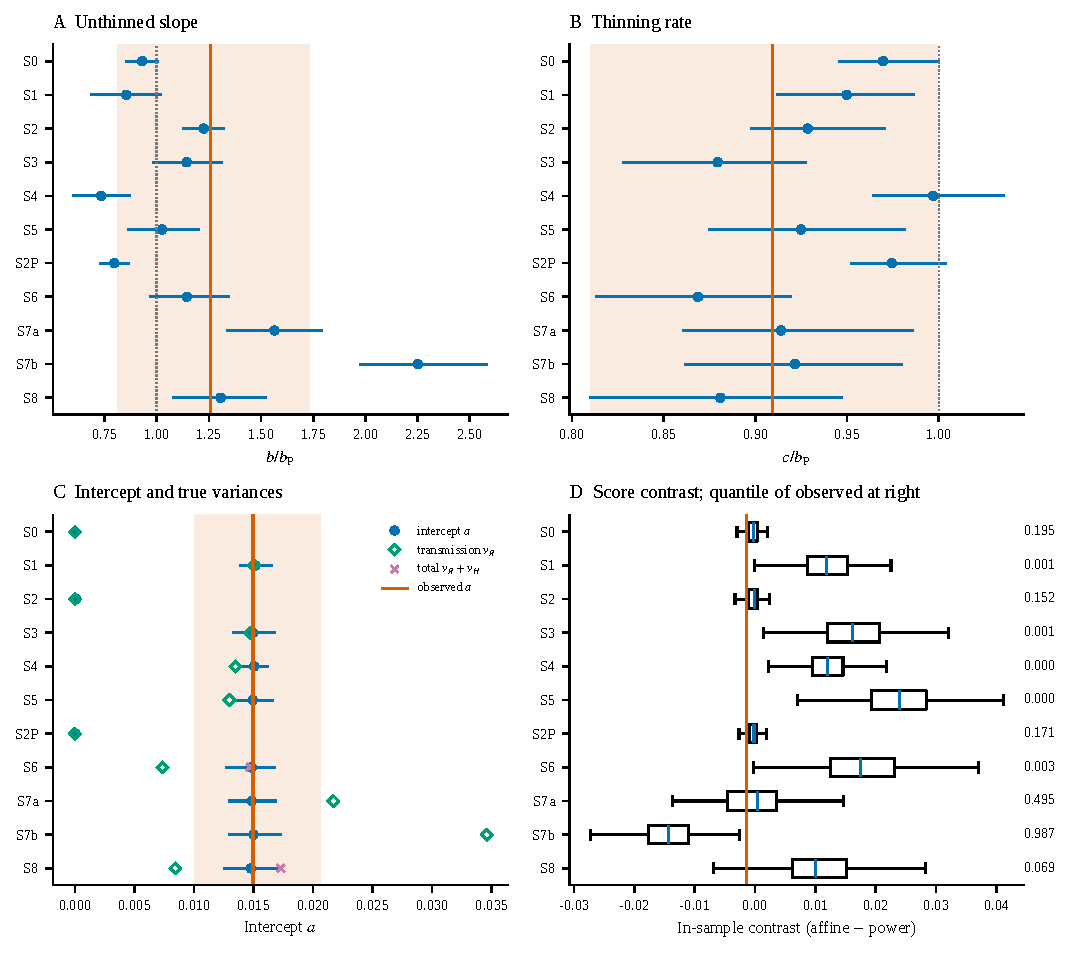
\includegraphics[width=0.95\linewidth]{figures/fig_09_audit.pdf}
\caption{Known-truth audit of the dispersion diagnostics on the real $R_A$ design, with simulated counts aligned to the observed median. Panel A shows the counting slope relative to the independent-Poisson reference, $b/\bP$, by generator. Panel B shows the thinning rate relative to the same reference, $c/\bP$. Panel C shows the fitted intercept $a$ against the true transmission relative variance and the true total, which differ only under S6 and S8. Panel D shows the in-sample score contrast between the affine and power-law fits, with the quantile of the observed value among synthetic panels at the right; boxes span the interquartile range and whiskers 1.5 times it. In panels A--C points are means over 200 panels per generator (100 panels for thinning) and bars are 2.5--97.5\% Monte Carlo ranges. The vertical line and shaded band mark the observed value and its bootstrap 95\% confidence interval; dotted lines mark 1. Generator labels are defined in Table~\ref{tab:ademp}; generator S9 is reported in Tables~\ref{tab:ma_tests} and~\ref{tab:ma_coverage}.}
\label{fig:audit}
\end{figure}

\FloatBarrier
\clearpage
\section{Supplementary tables and figures}
\label{app:supplement}
\renewcommand{\thetable}{S\arabic{table}}
\setcounter{table}{0}
\renewcommand{\thefigure}{S\arabic{figure}}
\setcounter{figure}{0}

Tables~\ref{tab:ma_baselines}--\ref{tab:ma_heldout_sim} give the slope references, the thinning check, the participation adjustment, the within-state slopes, the off-season reporting descriptors and the held-out comparison of curve shapes cited in the main text. Tables~\ref{tab:r2-deciles}--\ref{tab:r2-interval-types} give the decile fits, the state-structured generators, the clamp sensitivity of the wild bootstrap, the pigeonhole bootstrap under fresh-draw generators and the type of every interval quoted in the text. Table~\ref{tab:secondary} also reports the growth-factor statistic $G$ of the original analysis, which the revised analysis does not use, and season-specific fits with separate slopes, which differ from the common-slope season intercepts of Table~\ref{tab:rev_season_effects}.

\FloatBarrier
\begin{table}[htbp]
\centering
\small
\caption{Branching-Poisson and independent-Poisson slope references, analytic, simulated and observed}\label{tab:ma_baselines}
\setlength{\tabcolsep}{2pt}
\begin{tabularx}{\linewidth}{@{}>{\raggedright\arraybackslash}p{0.2400\linewidth}>{\raggedright\arraybackslash}p{0.1400\linewidth}>{\raggedright\arraybackslash}p{0.1400\linewidth}>{\raggedright\arraybackslash}p{0.1400\linewidth}>{\raggedright\arraybackslash}p{0.1400\linewidth}>{\raggedright\arraybackslash}p{0.1400\linewidth}@{}}
\toprule
Reference & Analytic reference / $b_P$ & Simulated b/$b_P$ (no heterogeneity) & MC SE & Simulated / analytic & Observed b / reference \\
\midrule
Branching-Poisson, $\rho$ = 0.1 & 0.944 & 0.877 [0.802, 0.955] & 0.0029 & 0.929 & 1.33 [0.86, 1.84] \\
Branching-Poisson, $\rho$ = 0.25 & 0.861 & 0.802 [0.734, 0.878] & 0.0026 & 0.932 & 1.46 [0.94, 2.02] \\
Branching-Poisson, $\rho$ = 0.5 & 0.722 & 0.669 [0.618, 0.714] & 0.0019 & 0.927 & 1.74 [1.12, 2.41] \\
Branching-Poisson, $\rho$ = 1 & 0.443 & 0.402 [0.373, 0.434] & 0.0012 & 0.907 & 2.84 [1.83, 3.94] \\
Independent-Poisson $b_P$ & 1 & 0.930 [0.853, 1.005] & 0.0029 & 0.930 & 1.26 [0.81, 1.73] \\
\bottomrule
\end{tabularx}
\par\smallskip
\begin{minipage}{\linewidth}\footnotesize\raggedright
The branching-Poisson reference is $b_{P,\mathrm{br}}$($\rho$) = mean over the observed retained rows of $\kappa^2$ [(1 - $\rho$) + ($C_t$ + 0.5)/($C_{t+1}$ + 0.5)]; independent-Poisson reference $b_P$ = 0.4455. Simulated rows use a pure branching chain with Poisson offspring and binomial reporting $\rho$ (independent-Poisson counts, S0, in the last row), no transmission heterogeneity, count-aligned as in the audit. Each has 200 panels, with the Monte Carlo 2.5-97.5\% range in brackets, and simulated / analytic is not normalised by the independent-Poisson row. The observed row uses the primary bootstrap (2,000 draws), with $b_{P,\mathrm{br}}$ recomputed with the weights of each draw. The ratio of the observed slope to the reference depends on the reporting probability.
\end{minipage}
\end{table}

\FloatBarrier
\begin{table}[htbp]
\centering
\small
\caption{Exact expected thinning increment against the delta prediction $b_P$}\label{tab:ma_thinning_exact}
\setlength{\tabcolsep}{2pt}
\begin{tabularx}{\linewidth}{@{}>{\raggedright\arraybackslash}p{0.2400\linewidth}>{\raggedright\arraybackslash}p{0.1400\linewidth}>{\raggedright\arraybackslash}p{0.1400\linewidth}>{\raggedright\arraybackslash}p{0.1400\linewidth}>{\raggedright\arraybackslash}p{0.1400\linewidth}>{\raggedright\arraybackslash}p{0.1400\linewidth}@{}}
\toprule
q & Exact rate & Exact rate / $b_P$ & MC rate [95\% CI] & Leverage in c & Positive-part mass (max) \\
\midrule
0.8 & 0.4672 & 1.049 & 0.4588 [0.3731, 0.5557] & 0.001 & 0.0e+00 \\
0.6 & 0.4845 & 1.087 & 0.4745 [0.4064, 0.5532] & 0.004 & 0.0e+00 \\
0.5 & 0.4957 & 1.113 & 0.4969 [0.4243, 0.5606] & 0.009 & 0.0e+00 \\
0.4 & 0.5050 & 1.133 & 0.4997 [0.4397, 0.5611] & 0.021 & 0.0e+00 \\
0.3 & 0.5051 & 1.134 & 0.5067 [0.4482, 0.5539] & 0.051 & 0.0e+00 \\
0.2 & 0.4798 & 1.077 & 0.4749 [0.4292, 0.5229] & 0.151 & 0.0e+00 \\
0.1 & 0.3836 & 0.861 & 0.3804 [0.3337, 0.4204] & 0.763 & 0.0e+00 \\
c, all q & 0.4084 & 0.917 & 0.4051 [0.3656, 0.4413] & 1.000 & -- \\
c, without q = 0.1 & 0.4882 & 1.096 & -- & -- & -- \\
\bottomrule
\end{tabularx}
\par\smallskip
\begin{minipage}{\linewidth}\footnotesize\raggedright
Rate = ($b_q$ - $b_1$)/(1/q - 1) from the affine FGLS fit of the exact expected thinned loss (binomial supports summed, mass below 1e-13 dropped); $b_P$ = 0.4455 is the delta-method prediction. Leverage is the share of the least-squares rate through the origin carried by each q. As a check, independent-thinning MC gives 0.4903 (SE 0.0048) against an expected-loss value of 0.4957 at q = 0.5, and 0.3832 (SE 0.0024) against 0.3836 at q = 0.1.
\end{minipage}
\end{table}

\FloatBarrier
\begin{table}[!tbp]
\centering
\scriptsize
\setlength{\tabcolsep}{3pt}
\caption{Shared-count binomial thinning of the $R_A$ sample (n=1748): summary by subset}
\label{tab:thinning}
\begin{tabularx}{\linewidth}{@{}ll*{5}{>{\centering\arraybackslash}X}@{}}
\toprule
Subset (n) & Fit over & $\bP$ [95\% CI] & $c$ [95\% CI] & $c/\bP$ [95\% CI] & $\Delta a$ rate $\times10^{3}$ [95\% CI] & $c/\bP$ by $q$, range \\
\midrule
full (1748) & all $q$ & 0.446 [0.428, 0.466] & 0.405 [0.366, 0.441] & 0.909 [0.810, 0.999] & -0.13 [-0.62, 0.47] & 0.85--1.14 \\
 & $q\ge0.2$ &  & 0.485 [0.439, 0.528] & 1.088 [0.994, 1.186] & -0.81 [-1.70, 0.05] & 1.03--1.14 \\
\addlinespace[2pt]
highCt50 (828) & all $q$ & 0.421 [0.403, 0.439] & 0.473 [0.409, 0.550] & 1.126 [0.970, 1.316] & -0.19 [-0.69, 0.15] & 1.05--1.14 \\
 & $q\ge0.2$ &  & 0.459 [0.381, 0.560] & 1.092 [0.903, 1.327] & -0.24 [-0.96, 0.21] & 1.05--1.10 \\
\addlinespace[2pt]
both50 (821) & all $q$ & 0.418 [0.401, 0.436] & 0.493 [0.420, 0.574] & 1.178 [1.004, 1.379] & -0.31 [-0.90, 0.10] & 1.16--1.21 \\
 & $q\ge0.2$ &  & 0.490 [0.397, 0.607] & 1.171 [0.953, 1.462] & -0.43 [-1.33, 0.12] & 1.16--1.21 \\
\bottomrule
\end{tabularx}
\par\smallskip
\begin{minipage}{\linewidth}\footnotesize\raggedright Thinning probabilities $q\in\{0.8, 0.6, 0.5, 0.4, 0.3, 0.2, 0.1\}$. $c$ is the increase of the slope per unit of $1/q-1$ and the $\Delta a$ rate the corresponding change of the intercept; $\bP$ is the independent-Poisson reference (plug-in delta value). highCt50 requires a current count of at least 50 and both50 both adjacent counts of at least 50; eligibility is fixed before thinning. Pairs bootstrap with B=1000 draws, 400 thinning replicates for the point estimate and 50 per bootstrap draw; the Monte Carlo precision criterion (MC SE at most 0.1 times the point estimate on the monitored summaries) is met; point fits 8400/8400, bootstrap fits 1049999/1050000. The last column gives the range of the per-$q$ point estimates of $c/\bP$ over the $q$ values of the fit. Per-$q$ estimates, simultaneous bands over $q$ and leave-one-$q$-out fits are in the released file analysis/authors/thinning.json.\end{minipage}
\end{table}

\FloatBarrier
\begingroup\scriptsize\setlength{\tabcolsep}{2pt}
\begin{longtable}{@{}>{\raggedright\arraybackslash}p{\dimexpr 0.2400\linewidth-3.500pt\relax}>{\raggedright\arraybackslash}p{\dimexpr 0.1000\linewidth-3.500pt\relax}>{\raggedright\arraybackslash}p{\dimexpr 0.1000\linewidth-3.500pt\relax}>{\raggedright\arraybackslash}p{\dimexpr 0.1000\linewidth-3.500pt\relax}>{\raggedright\arraybackslash}p{\dimexpr 0.1000\linewidth-3.500pt\relax}>{\raggedright\arraybackslash}p{\dimexpr 0.1000\linewidth-3.500pt\relax}>{\raggedright\arraybackslash}p{\dimexpr 0.1000\linewidth-3.500pt\relax}>{\raggedright\arraybackslash}p{\dimexpr 0.1000\linewidth-3.500pt\relax}@{}}
\caption{Small-count variance of the log thinned count relative to the delta approximation}\label{tab:ma_varlog}\\
\toprule
C & q = 0.8 & q = 0.6 & q = 0.5 & q = 0.4 & q = 0.3 & q = 0.2 & q = 0.1 \\
\midrule
\endfirsthead
\multicolumn{8}{@{}l}{\textit{(continued)}}\\
\toprule
C & q = 0.8 & q = 0.6 & q = 0.5 & q = 0.4 & q = 0.3 & q = 0.2 & q = 0.1 \\
\midrule
\endhead
\midrule
\multicolumn{8}{r@{}}{\textit{(continued on next page)}}\\
\endfoot
\bottomrule
\endlastfoot
5 & 1.05 & 1.11 & 1.11 & 1.04 & 0.86 & 0.57 & 0.21 \\
10 & 1.02 & 1.05 & 1.08 & 1.12 & 1.13 & 0.99 & 0.53 \\
20 & 1.01 & 1.02 & 1.03 & 1.05 & 1.09 & 1.14 & 0.97 \\
45 & 1.00 & 1.01 & 1.01 & 1.02 & 1.03 & 1.06 & 1.14 \\
100 & 1.00 & 1.00 & 1.01 & 1.01 & 1.01 & 1.02 & 1.06 \\
500 & 1.00 & 1.00 & 1.00 & 1.00 & 1.00 & 1.00 & 1.01 \\
\end{longtable}
\vspace{-.5\baselineskip}
\noindent\begin{minipage}{\linewidth}\footnotesize\raggedright
Exact added variance Var log(Bin(C, q) + 0.5) - Var log(C + 0.5) divided by the delta value (1 - q)/(qC). Values below 1 mean that thinning adds less variance than the delta method assumes.
\end{minipage}\par
\endgroup

\FloatBarrier
\begin{figure}[!tbp]
\centering
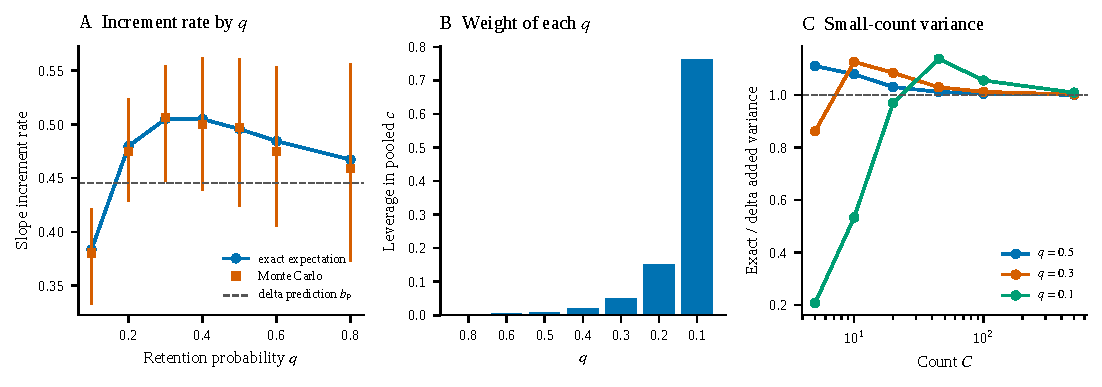
\includegraphics[width=0.98\linewidth]{figures/fig_10_thinning_exact.pdf}
\caption{Exact thinning expectation on the observed counts. Panel A shows the expected increment rate of the inverse-count slope by retention probability $q$, exact expectation against Monte Carlo estimates with 95\% ranges; the dashed line is the delta prediction $\bP=0.4455$. Panel B shows the share of each $q$ in the leverage of the pooled least-squares rate $c$. Panel C shows the exact added variance of the log thinned count relative to its delta approximation, by original count $C$, for three retention probabilities.}
\label{fig:thinning-exact}
\end{figure}
\clearpage
\begingroup\scriptsize\setlength{\tabcolsep}{2pt}
\begin{longtable}{@{}>{\raggedright\arraybackslash}p{\dimexpr 0.2400\linewidth-3.333pt\relax}>{\raggedright\arraybackslash}p{\dimexpr 0.1400\linewidth-3.333pt\relax}>{\raggedright\arraybackslash}p{\dimexpr 0.1400\linewidth-3.333pt\relax}>{\raggedright\arraybackslash}p{\dimexpr 0.1400\linewidth-3.333pt\relax}>{\raggedright\arraybackslash}p{\dimexpr 0.1400\linewidth-3.333pt\relax}>{\raggedright\arraybackslash}p{\dimexpr 0.1400\linewidth-3.333pt\relax}@{}}
\caption{Season-specific fits and reporting participation sensitivity}\label{tab:secondary}\\
\toprule
Statistic / period & n & a / change [95\% CI] & b / original a & b/a / adjusted a & Finite/B \\
\midrule
\endfirsthead
\multicolumn{6}{@{}l}{\textit{(continued)}}\\
\toprule
Statistic / period & n & a / change [95\% CI] & b / original a & b/a / adjusted a & Finite/B \\
\midrule
\endhead
\midrule
\multicolumn{6}{r@{}}{\textit{(continued on next page)}}\\
\endfoot
\bottomrule
\endlastfoot
RA / 2022-23 & 365 & 0.01369 [0.0071, 0.02102] & 0.6967 & 50.91 & 1000/1000 \\
RA / 2023-24 & 499 & 0.006174 [0.002667, 0.01542] & 0.7018 & 113.7 & 1000/1000 \\
RA / 2024-25 & 356 & 0.01268 [0.005687, 0.02276] & 0.5826 & 45.93 & 1000/1000 \\
RA / 2025-26 & 528 & 0.02253 [0.008432, 0.03509] & 0.3533 & 15.68 & 1000/1000 \\
RA / reporting adjustment & 1748 & 0.0002939 [-0.0003183, 0.0008476] & 0.01495 & 0.01466 & 1000/1000 \\
G / 2022-23 & 367 & 0.07179 [0.03786, 0.1162] & 2.702 & 37.64 & 1000/1000 \\
G / 2023-24 & 503 & 0.03046 [0.0118, 0.07462] & 2.382 & 78.2 & 1000/1000 \\
G / 2024-25 & 357 & 0.06469 [0.03191, 0.1278] & 2.082 & 32.19 & 1000/1000 \\
G / 2025-26 & 529 & 0.1383 [0.03715, 0.2252] & 0.7411 & 5.359 & 1000/1000 \\
G / reporting adjustment & 1756 & 0.000373 [-0.003559, 0.003454] & 0.08401 & 0.08364 & 1000/1000 \\
\end{longtable}
\vspace{-.5\baselineskip}
\noindent\begin{minipage}{\linewidth}\footnotesize\raggedright
Season rows report a with its interval and b, b/a as point estimates only. Reporting-adjustment rows use the a column for original-minus-adjusted a [95\% CI], b for original a, and b/a for adjusted a; the original normalizer is fixed. Season b and b/a come from separate per-season fits without a stored bootstrap; season b/a with intervals from a common-slope model are given in the season table. Summer rows are reported in a separate table. All 1,000 draws were finite in every season for RA and G. Season intervals here use 1,000 draws and those of Table~\ref{tab:ma_sensitivity} 2,000, so their limits differ slightly.
\end{minipage}\par
\endgroup

\clearpage
\begingroup\scriptsize\setlength{\tabcolsep}{2pt}
\begin{longtable}{@{}>{\raggedright\arraybackslash}p{\dimexpr 0.2400\linewidth-3.200pt\relax}>{\raggedright\arraybackslash}p{\dimexpr 0.1750\linewidth-3.200pt\relax}>{\raggedright\arraybackslash}p{\dimexpr 0.1750\linewidth-3.200pt\relax}>{\raggedright\arraybackslash}p{\dimexpr 0.1750\linewidth-3.200pt\relax}>{\raggedright\arraybackslash}p{\dimexpr 0.1750\linewidth-3.200pt\relax}@{}}
\caption{Within-state, within-week and two-way slopes against the independent-Poisson reference (bootstrap 95\% confidence interval in brackets)}\label{tab:ma_within}\\
\toprule
Estimator & Slope [95\% CI] & Slope / $b_P$ & Slope / pooled b & Fit status \\
\midrule
\endfirsthead
\multicolumn{5}{@{}l}{\textit{(continued)}}\\
\toprule
Estimator & Slope [95\% CI] & Slope / $b_P$ & Slope / pooled b & Fit status \\
\midrule
\endhead
\midrule
\multicolumn{5}{r@{}}{\textit{(continued on next page)}}\\
\endfoot
\bottomrule
\endlastfoot
Pooled affine slope b & 0.560 [0.362, 0.769] & 1.26 [0.81, 1.73] & -- & -- \\
$b_P$, independent-Poisson reference & 0.446 [0.427, 0.465] & -- & -- & -- \\
State FE, iterated FGLS ($b_w$) & 0.379 [0.107, 0.650] & 0.85 [0.24, 1.47] & 0.68 [0.26, 1.01] & -- \\
State FE, one-step WLS & 0.456 [0.228, 0.682] & 1.02 [0.51, 1.53] & 0.81 [0.57, 0.96] & single step \\
Week FE, one-step WLS & 0.634 [0.420, 0.846] & 1.42 [0.96, 1.89] & 1.13 [0.98, 1.34] & single step \\
State + week FE, one-step WLS & 0.480 [0.208, 0.744] & 1.08 [0.47, 1.66] & 0.86 [0.47, 1.14] & single step \\
State + week FE, damped iterated FGLS & 0.414 [0.040, 0.659] & 0.93 [0.09, 1.48] & 0.74 [0.09, 1.10] & converged, 124 it. \\
\end{longtable}
\vspace{-.5\baselineskip}
\noindent\begin{minipage}{\linewidth}\footnotesize\raggedright
The primary bootstrap uses the state-week weights of the primary stream with 2,000 draws, so the pooled row equals Table~\ref{tab:pooled}; draws whose iterated fit does not converge are dropped (1962 valid for the damped two-way slope). The undamped two-way iteration did not converge after 51 iterations (last values 0.4150, 0.4122); damping 0.5 removes the two-cycle. One-step WLS uses the pooled affine working precision; the iterated estimators re-weight with the fixed-effect fitted means.
\end{minipage}\par
\endgroup

\FloatBarrier
\begin{table}[H]
\centering
\small
\caption{Off-season summer descriptors}\label{tab:summer}
\setlength{\tabcolsep}{2pt}
\begin{tabularx}{\linewidth}{@{}>{\raggedright\arraybackslash}p{0.2400\linewidth}>{\raggedright\arraybackslash}p{0.1750\linewidth}>{\raggedright\arraybackslash}p{0.1750\linewidth}>{\raggedright\arraybackslash}p{0.1750\linewidth}>{\raggedright\arraybackslash}p{0.1750\linewidth}@{}}
\toprule
Period & n & Median count scale & Median participation (\%) & IQR(log G) \\
\midrule
Summer 2023 & 772 & 15.55 & 94.24 & 0.4873 \\
Summer 2024 & 400 & 17.12 & 45.59 & 0.6683 \\
Summer 2025 & 839 & 16.25 & 92.31 & 0.4882 \\
\bottomrule
\end{tabularx}
\par\smallskip
\noindent\begin{minipage}{\linewidth}\footnotesize\raggedright
Descriptive summaries of May-October state-weeks with $D_t$ $\ge$ 5: rows, median count scale $D_t$, median reporting participation (\%) and IQR of log G. No model is fitted, so no interval is given. Reporting was voluntary in the 2024 summer only; that contrast is descriptive, not a causal or independently replicated intervention.
\end{minipage}
\end{table}

\clearpage
\begingroup\scriptsize\setlength{\tabcolsep}{2pt}
\begin{longtable}{@{}>{\raggedright\arraybackslash}p{\dimexpr 0.2400\linewidth-3.500pt\relax}>{\raggedright\arraybackslash}p{\dimexpr 0.1000\linewidth-3.500pt\relax}>{\raggedright\arraybackslash}p{\dimexpr 0.1000\linewidth-3.500pt\relax}>{\raggedright\arraybackslash}p{\dimexpr 0.1000\linewidth-3.500pt\relax}>{\raggedright\arraybackslash}p{\dimexpr 0.1000\linewidth-3.500pt\relax}>{\raggedright\arraybackslash}p{\dimexpr 0.1000\linewidth-3.500pt\relax}>{\raggedright\arraybackslash}p{\dimexpr 0.1000\linewidth-3.500pt\relax}>{\raggedright\arraybackslash}p{\dimexpr 0.1000\linewidth-3.500pt\relax}@{}}
\caption{Held-out comparison of the affine and power loss models with paired uncertainty}\label{tab:ma_validation}\\
\toprule
Held-out unit & Folds & Mean power - affine score & Paired fold SE & z & Folds favouring affine & Bootstrap 95\% CI & Bootstrap share favouring affine \\
\midrule
\endfirsthead
\multicolumn{8}{@{}l}{\textit{(continued)}}\\
\toprule
Held-out unit & Folds & Mean power - affine score & Paired fold SE & z & Folds favouring affine & Bootstrap 95\% CI & Bootstrap share favouring affine \\
\midrule
\endhead
\midrule
\multicolumn{8}{r@{}}{\textit{(continued on next page)}}\\
\endfoot
\bottomrule
\endlastfoot
State & 51 & -0.0020 & 0.0068 & -0.30 & 26/51 & [-0.0290, 0.0298] & 0.43 \\
Season & 4 & 0.0046 & 0.0087 & 0.53 & 3/4 & [-0.0295, 0.0655] & 0.54 \\
\end{longtable}
\vspace{-.5\baselineskip}
\noindent\begin{minipage}{\linewidth}\footnotesize\raggedright
Score: weighted mean of L/mu + log mu on held-out rows; positive differences favour the affine model. Paired fold SE from the between-fold variation of the paired differences; state-week bootstrap with 1000 draws refits both models in every fold.
\end{minipage}\par
\endgroup


\begingroup\let\oldtable\table\renewcommand{\table}[1][]{\oldtable[!h]}
\begin{table}[!tbp]
\centering
\scriptsize
\setlength{\tabcolsep}{3pt}
\caption{Held-out power-minus-affine score contrast on synthetic panels from each generator}
\label{tab:ma_heldout_sim}
\begin{tabularx}{\linewidth}{@{}l*{6}{>{\centering\arraybackslash}X}@{}}
\toprule
 & \multicolumn{3}{c}{Leave one state out (51 folds)} & \multicolumn{3}{c}{Leave one season out (4 folds)} \\
\cmidrule(lr){2-4}\cmidrule(l){5-7}
Generator & Mean contrast ($\times10^{3}$) & Affine better & Observed quantile & Mean contrast ($\times10^{3}$) & Affine better & Observed quantile \\
Observed & -2.02 & & & 4.63 & & \\
\midrule
S0 & -1.01 (0.19) & 0.34 & 0.235 (0.030) & -0.89 (0.23) & 0.38 & 0.970 (0.012) \\
S1 & 12.84 (0.37) & 0.99 & 0.000 (0.000) & 12.97 (0.37) & 0.99 & 0.060 (0.017) \\
S2 & -0.21 (0.13) & 0.51 & 0.125 (0.023) & -0.09 (0.15) & 0.50 & 0.985 (0.009) \\
S2P & -1.00 (0.18) & 0.35 & 0.215 (0.029) & -0.81 (0.31) & 0.42 & 0.980 (0.010) \\
S3 & 17.38 (0.44) & 1.00 & 0.000 (0.000) & 17.49 (0.44) & 1.00 & 0.000 (0.000) \\
S4 & 11.21 (0.36) & 0.99 & 0.000 (0.000) & 15.78 (0.38) & 1.00 & 0.010 (0.007) \\
S5 & 24.03 (0.48) & 1.00 & 0.000 (0.000) & 28.32 (0.58) & 1.00 & 0.000 (0.000) \\
S6 & 18.74 (0.59) & 0.99 & 0.000 (0.000) & 18.60 (0.58) & 0.99 & 0.045 (0.015) \\
S7a & -1.32 (0.44) & 0.41 & 0.475 (0.035) & -0.85 (0.44) & 0.44 & 0.805 (0.028) \\
S7b & -15.42 (0.38) & 0.00 & 0.995 (0.005) & -14.31 (0.40) & 0.01 & 1.000 (0.000) \\
S8 & 11.07 (0.60) & 0.91 & 0.050 (0.015) & 11.15 (0.62) & 0.91 & 0.220 (0.029) \\
S9 & 11.83 (0.59) & 0.92 & 0.055 (0.016) & 12.60 (0.62) & 0.93 & 0.145 (0.025) \\
\bottomrule
\end{tabularx}
\par\smallskip
\begin{minipage}{\linewidth}\footnotesize\raggedright 200 synthetic panels per generator, each analysed with the fold design and score of the data: mean of $L/\mu+\log\mu$ on the held-out rows, weighted by rows, power law minus affine (positive values favour the affine form). Mean contrast with its Monte Carlo standard error; affine better, share of panels with a positive contrast; observed quantile, share of panels with a contrast at or below the observed one, with binomial Monte Carlo standard error.\end{minipage}
\end{table}

\endgroup
\FloatBarrier
\clearpage
\begin{table}[!tbp]
\centering
\scriptsize\renewcommand{\arraystretch}{1.15}
\setlength{\tabcolsep}{3pt}
\caption{Observed and fitted loss by decile of the current-week count}
\label{tab:r2-deciles}
\begin{tabularx}{\linewidth}{@{}rrrrrlrrrr@{}}
\toprule
Decile & $C_t$ & $n$ & Mean $C_t$ & Mean $L$ & 95\% interval & Affine & Power & Three-par. & Affine inside \\
\midrule
1 & 5--10 & 188 & 7.8 & 0.0684 & 0.0538--0.0854 & 0.0906 & 0.0656 & 0.0748 & no \\
2 & 11--15 & 180 & 13.0 & 0.0597 & 0.0425--0.0787 & 0.0584 & 0.0533 & 0.0559 & yes \\
3 & 16--21 & 162 & 18.4 & 0.0557 & 0.0431--0.0699 & 0.0457 & 0.0467 & 0.0469 & yes \\
4 & 22--32 & 176 & 26.7 & 0.0321 & 0.0249--0.0404 & 0.0362 & 0.0405 & 0.0392 & yes \\
5 & 33--45 & 173 & 38.5 & 0.0404 & 0.0310--0.0501 & 0.0296 & 0.0352 & 0.0330 & no \\
6 & 46--73 & 174 & 57.4 & 0.0228 & 0.0174--0.0292 & 0.0249 & 0.0303 & 0.0278 & yes \\
7 & 74--116 & 171 & 93.5 & 0.0223 & 0.0166--0.0287 & 0.0210 & 0.0251 & 0.0229 & yes \\
8 & 117--206 & 174 & 153.4 & 0.0191 & 0.0144--0.0241 & 0.0187 & 0.0208 & 0.0193 & yes \\
9 & 207--388 & 175 & 274.2 & 0.0190 & 0.0132--0.0249 & 0.0171 & 0.0167 & 0.0162 & yes \\
10 & 390--3870 & 175 & 881.9 & 0.0110 & 0.0079--0.0137 & 0.0158 & 0.0115 & 0.0130 & no \\
\bottomrule
\end{tabularx}
\par\smallskip\parbox{\linewidth}{\scriptsize\linespread{1.15}\selectfont Rows of $R_A$ (1,748) split at the deciles of the current-week count $C_t$. Mean $L$: observed mean relative squared deviation; 95\% interval from a calendar-week block bootstrap (1,999 draws). Model columns give the mean prediction in the decile under the affine fit $a+b/C$ ($a=0.0150$, $b=0.560$), the power law $cC^{-\gamma}$ ($\gamma=0.383$) and the three-parameter fit $a+bC^{-\gamma}$ ($a=0.0089$, $\gamma=0.617$). Quasi-deviance: affine -4346.2, power -4348.6, three-parameter -4356.9. Last column: whether the affine prediction lies inside the interval of the observed mean.}
\end{table}

\FloatBarrier
\begin{table}[!tbp]
\centering
\scriptsize\renewcommand{\arraystretch}{1.15}
\setlength{\tabcolsep}{3pt}
\caption{State-realistic fresh-draw generators against four features of the observed panel}
\label{tab:r2-generator}
\begin{tabularx}{\linewidth}{@{}Xlllllrrr@{}}
\toprule
Cell & $\sigma$ & T1 $b/b_P$ & T2 P90 & T3 pooled/within & T4 state CV & $E(\hat a)/v_R$ & SE/SD & Coverage \\
\midrule
SR-pop-c0 & failed & 1.06--1.43 & 367 & 1.07--1.47* & 0.41--0.72 & 1.24 & 2.31 & 1.000 \\
SR-pop-c25 & failed & 1.35--1.89* & 364 & 1.02--1.34* & 0.47--0.78 & 1.26 & 1.79 & 0.990 \\
SR-pop-c50 & failed & 1.67--2.21* & 356 & 1.03--1.31* & 0.52--0.93 & 1.25 & 1.81 & 0.990 \\
SR-fe-c25 & failed & 1.45--1.93* & 364 & 1.04--1.41* & 0.55--0.90 & 1.26 & 1.78 & 0.990 \\
SR-pop-c25-r003 & failed & 1.38--1.84* & 363 & 1.02--1.34* & 0.46--0.76 & 1.27 & 1.80 & 1.000 \\
SR-pop-c25-t50 & 0.161 & 1.29--1.77* & 308* & 1.04--1.39* & 0.47--0.93 & 1.56 & 1.63 & 0.960 \\
Observed & -- & 1.26 & 389 & 1.48 & 0.59 & -- & -- & -- \\
\bottomrule
\end{tabularx}
\par\smallskip\parbox{\linewidth}{\scriptsize\linespread{1.15}\selectfont State-realistic generators (200 panels per cell): transmission field around a smoothed observed trend with state-specific variance (multiplier proportional to the population-dependent intercept, or to the state fixed-effect intercepts for SR-fe), clustered admissions with extra-Poisson parameter $\theta_c$ (c0, c25, c50 $=0, 0.25, 0.5$), reporting probability 0.01 (0.003 for r003), trend exponent 1 (0.5 for t50). $\sigma$: transmission SD scale; ``failed'' when the smoothed trend alone exceeds the transmission target ($\sigma=0$). T1--T4: Monte Carlo 2.5--97.5\% range of $b/b_P$, mean P90 of $C_t$ (band 350--428), range of pooled/within slope ratio and of the between-state CV of intercepts; * the observed value lies outside. Success rule of Amendment 2: all four pass in one cell (outcome: M4/M5 unresolved). Last columns: $E(\hat a)/v_R$, observed SE over Monte Carlo SD of $\hat a$, coverage of $E(\hat a)$ by the two-way interval. Data-informed generator design; no inferential result uses these generators.}
\end{table}

\FloatBarrier
\begin{table}[!tbp]
\centering
\scriptsize\renewcommand{\arraystretch}{1.15}
\setlength{\tabcolsep}{3pt}
\caption{Wild bootstrap of the intercept under alternative loss clamps}
\label{tab:r2-clamp}
\begin{tabularx}{\linewidth}{@{}Xrllll@{}}
\toprule
Variant & Valid draws & $p$ (two-sided) & Min.\ $p$ & Clamped rows (\%) & $t^*$ quantiles \\
\midrule
clamp at $10^{-9}$ & 9,999 & 0.0001 & 0.0001 & 13.5 & $-$0.15 / 1.80 / 3.38 \\
clamp at $10^{-7}$ (primary) & 9,999 & 0.0001 & 0.0001 & 13.5 & $-$0.15 / 1.80 / 3.38 \\
clamp at $10^{-5}$ & 9,999 & 0.0001 & 0.0001 & 13.8 & $-$0.16 / 1.80 / 3.38 \\
clamp at $10^{-3}$ & 9,999 & 0.0001 & 0.0001 & 17.0 & 0.43 / 2.03 / 3.53 \\
no clamp & 3,768 & 0.0003 & 0.0003 & 13.5 & 0.32 / 1.11 / 2.88 \\
exclude draws with any clamped row & 0 & not evaluable & -- & -- & -- \\
\bottomrule
\end{tabularx}
\par\smallskip\parbox{\linewidth}{\scriptsize\linespread{1.15}\selectfont Wild cluster bootstrap-$t$ of the intercept (9,999 draws, calendar-week Webb weights, seed 21); $t_{\mathrm{obs}}=7.36$. Valid: draws with a converged fit. Minimum attainable $p$: $1/(\text{valid}+1)$. Clamped rows: share of bootstrap rows whose loss is at or below the clamp (for no clamp: negative losses, kept). $t^*$: 2.5\%, 50\%, 97.5\% quantiles. Every draw contains at least one clamped row, so the exclusion variant has no draws. Secondary calibration; it does not change the E1 verdict.}
\end{table}

\FloatBarrier
\begin{table}[!tbp]
\centering
\scriptsize\renewcommand{\arraystretch}{1.15}
\setlength{\tabcolsep}{3pt}
\caption{Pigeonhole bootstrap SD of the intercept against the Monte Carlo SD}
\label{tab:r2-bootstrap-sd}
\begin{tabularx}{\linewidth}{@{}Xrrrlrr@{}}
\toprule
Generator & Panels & MC SD ($\times10^3$) & Boot.\ SD ($\times10^3$) & Boot./MC & Sandwich/MC & Coverage \\
\midrule
FD-S1 & 100 & 0.976 & 1.742 & 1.78 (1.47--2.22) & 1.02 & 1.00 \\
FD-S8 & 100 & 1.266 & 2.121 & 1.67 (1.29--2.07) & 0.92 & 0.99 \\
FD-S9-25$^\dagger$ & 100 & 1.300 & 2.148 & 1.65 (1.29--2.05) & 0.94 & 1.00 \\
FD-S9-50$^\dagger$ & 100 & 1.324 & 2.196 & 1.66 (1.28--2.22) & 1.03 & 1.00 \\
FD-S9-75$^\dagger$ & 100 & 1.465 & 2.270 & 1.55 (1.19--1.92) & 1.07 & 0.99 \\
\bottomrule
\end{tabularx}
\par\smallskip\parbox{\linewidth}{\scriptsize\linespread{1.15}\selectfont Pigeonhole (state $\times$ calendar-week) bootstrap, 199 draws per panel, on the first 100 stored panels of each fresh-draw generator (panels regenerated exactly from the stored seeds). MC SD: Monte Carlo SD of $\hat a$ over 200 panels. Ratio range over panels in brackets. Sandwich: two-way SE over MC SD. Coverage: share of panels whose percentile interval covers $E(\hat a)$. $^\dagger$ post hoc law. Reading rule of Amendment 2: conservative if every ratio exceeds 1 (outcome: conservative).}
\end{table}

\FloatBarrier
\begin{table}[!tbp]
\centering
\tiny
\setlength{\tabcolsep}{3pt}
\caption{Type and source of every interval quoted in the manuscript}
\label{tab:r2-interval-types}
\begin{tabularx}{\linewidth}{@{}p{0.11\linewidth}p{0.2\linewidth}lp{0.25\linewidth}X@{}}
\toprule
Location & Quantity & Quoted & Type & Source \\
\midrule
Abstract; Results: count-independent floor & a, pooled affine intercept (primary test) & 0.0109--0.0191 & two-way CGM sandwich (state x calendar week), t with G-1 = 41 df & {\ttfamily\tiny results.\allowbreak{}json.\allowbreak{}revision\_2026\_11.\allowbreak{}E1\_intercept.\allowbreak{}primary.\allowbreak{}inference.\allowbreak{}two\_way.\allowbreak{}a\_ci} \\
Results: count-independent floor & b, counting slope & 0.430--0.690 & two-way CGM sandwich (state x calendar week), t with G-1 = 41 df & {\ttfamily\tiny results.\allowbreak{}json.\allowbreak{}revision\_2026\_11.\allowbreak{}E1\_intercept.\allowbreak{}primary.\allowbreak{}inference.\allowbreak{}two\_way.\allowbreak{}b\_ci} \\
Results: count-independent floor & a, clustering by state only & 0.0125--0.0174 & one-way CGM sandwich by state, t with 50 df & {\ttfamily\tiny results.\allowbreak{}json.\allowbreak{}revision\_2026\_11.\allowbreak{}E1\_intercept.\allowbreak{}primary.\allowbreak{}inference.\allowbreak{}state.\allowbreak{}a\_ci} \\
Results: count-independent floor & a, clustering by calendar week only & 0.0112--0.0188 & one-way CGM sandwich by calendar week, t with 41 df & {\ttfamily\tiny results.\allowbreak{}json.\allowbreak{}revision\_2026\_11.\allowbreak{}E1\_intercept.\allowbreak{}primary.\allowbreak{}inference.\allowbreak{}week.\allowbreak{}a\_ci} \\
Results: count-independent floor & a, block bootstrap & 0.0107--0.0192 & calendar-week block bootstrap percentile (1,999 draws) & {\ttfamily\tiny results.\allowbreak{}json.\allowbreak{}revision\_2026\_11.\allowbreak{}E1\_intercept.\allowbreak{}block\_bootstrap.\allowbreak{}a.\allowbreak{}ci} \\
Results: count-independent floor & a, point estimates over 17 specifications & 0.0117--0.0202 & range of point values (not an interval) & {\ttfamily\tiny results.\allowbreak{}json.\allowbreak{}revision\_2026\_11.\allowbreak{}E1\_intercept.\allowbreak{}sensitivities.\allowbreak{}*.\allowbreak{}a (min and max)} \\
Results: count-independent floor & a at C\_t >= 50 & 0.0088--0.0172 & two-way CGM sandwich (state x calendar week), t with G-1 = 41 df & {\ttfamily\tiny results.\allowbreak{}json.\allowbreak{}revision\_2026\_11.\allowbreak{}E1\_intercept.\allowbreak{}sensitivities.\allowbreak{}S-a3\_floor\_50.\allowbreak{}inference.\allowbreak{}two\_way.\allowbreak{}a\_ci} \\
Results: count-independent floor & a, fixed calendar windows & 0.0092--0.0311 & two-way CGM sandwich (state x calendar week), t with G-1 = 41 df & {\ttfamily\tiny results.\allowbreak{}json.\allowbreak{}revision\_2026\_11.\allowbreak{}E1\_intercept.\allowbreak{}sensitivities.\allowbreak{}S-a4\_calendar\_windows.\allowbreak{}inference.\allowbreak{}two\_way.\allowbreak{}a\_ci} \\
Results: count-independent floor & a, leave-one-week-out point estimates & 0.0136--0.0156 & range of point values (not an interval) & {\ttfamily\tiny results.\allowbreak{}json.\allowbreak{}revision\_2026\_11.\allowbreak{}E1\_intercept.\allowbreak{}sensitivities.\allowbreak{}S-a9\_leave\_one\_week\_out (min and max)} \\
Results: fit of the affine form & mean L, lowest count decile & 0.0538--0.0854 & calendar-week block bootstrap percentile (1,999 draws) & {\ttfamily\tiny results.\allowbreak{}json.\allowbreak{}revision\_2026\_11\_r2.\allowbreak{}B\_floor.\allowbreak{}B1\_deciles.\allowbreak{}rows\allowbreak{}[0].\allowbreak{}mean\_L\_ci} \\
Results: fit of the affine form & mean L, highest count decile & 0.0079--0.0137 & calendar-week block bootstrap percentile (1,999 draws) & {\ttfamily\tiny results.\allowbreak{}json.\allowbreak{}revision\_2026\_11\_r2.\allowbreak{}B\_floor.\allowbreak{}B1\_deciles.\allowbreak{}rows\allowbreak{}[9].\allowbreak{}mean\_L\_ci} \\
Results: fit of the affine form & mean L, fifth count decile & 0.0310--0.0501 & calendar-week block bootstrap percentile (1,999 draws) & {\ttfamily\tiny results.\allowbreak{}json.\allowbreak{}revision\_2026\_11\_r2.\allowbreak{}B\_floor.\allowbreak{}B1\_deciles.\allowbreak{}rows\allowbreak{}[4].\allowbreak{}mean\_L\_ci} \\
Results: fit of the affine form & gamma, three-parameter fit, week bootstrap & 0.355--0.870 & calendar-week block bootstrap percentile (1,999 draws) & {\ttfamily\tiny results.\allowbreak{}json.\allowbreak{}revision\_2026\_11\_r2.\allowbreak{}B\_floor.\allowbreak{}B3\_three\_parameter.\allowbreak{}week\_bootstrap.\allowbreak{}gamma.\allowbreak{}ci} \\
Results: fit of the affine form & gamma, three-parameter fit, state bootstrap & 0.438--0.862 & state bootstrap percentile (states resampled) (999 draws) & {\ttfamily\tiny results.\allowbreak{}json.\allowbreak{}revision\_2026\_11\_r2.\allowbreak{}B\_floor.\allowbreak{}B3\_three\_parameter.\allowbreak{}state\_bootstrap.\allowbreak{}gamma.\allowbreak{}ci} \\
Results: fit of the affine form & a, three-parameter fit, week bootstrap & $-$0.0014 to 0.0137 & calendar-week block bootstrap percentile (1,999 draws) & {\ttfamily\tiny results.\allowbreak{}json.\allowbreak{}revision\_2026\_11\_r2.\allowbreak{}B\_floor.\allowbreak{}B3\_three\_parameter.\allowbreak{}week\_bootstrap.\allowbreak{}a.\allowbreak{}ci} \\
Results: fit of the affine form & a, three-parameter fit, state bootstrap & 0.0034--0.0144 & state bootstrap percentile (states resampled) (999 draws) & {\ttfamily\tiny results.\allowbreak{}json.\allowbreak{}revision\_2026\_11\_r2.\allowbreak{}B\_floor.\allowbreak{}B3\_three\_parameter.\allowbreak{}state\_bootstrap.\allowbreak{}a.\allowbreak{}ci} \\
Results: fit of the affine form & mean L, rows at or above P90 & 0.0078--0.0139 & calendar-week block bootstrap percentile (1,999 draws) & {\ttfamily\tiny results.\allowbreak{}json.\allowbreak{}revision\_2026\_11\_r2.\allowbreak{}B\_floor.\allowbreak{}B4\_model\_free\_floor.\allowbreak{}rows\allowbreak{}[1].\allowbreak{}mean\_L\_ci} \\
Abstract; Results: fit of the affine form & relative RMSE, rows at or above P90 (\%) & 8.8--11.8 & calendar-week block bootstrap percentile (1,999 draws) & {\ttfamily\tiny results.\allowbreak{}json.\allowbreak{}revision\_2026\_11\_r2.\allowbreak{}B\_floor.\allowbreak{}B4\_model\_free\_floor.\allowbreak{}rows\allowbreak{}[1].\allowbreak{}rel\_rmse\_ci} \\
Results: fit of the affine form & floor L - b\_hat/C, P90 & 0.0069--0.0132 & calendar-week block bootstrap percentile (1,999 draws) & {\ttfamily\tiny results.\allowbreak{}json.\allowbreak{}revision\_2026\_11\_r2.\allowbreak{}B\_floor.\allowbreak{}B4\_model\_free\_floor.\allowbreak{}rows\allowbreak{}[1].\allowbreak{}floor\_minus\_bhat\_ci} \\
Results: fit of the affine form & floor relative SD, P90 (\%) & 8.3--11.5 & calendar-week block bootstrap percentile (1,999 draws) & {\ttfamily\tiny results.\allowbreak{}json.\allowbreak{}revision\_2026\_11\_r2.\allowbreak{}B\_floor.\allowbreak{}B4\_model\_free\_floor.\allowbreak{}rows\allowbreak{}[1].\allowbreak{}floor\_rel\_sd\_bhat\_ci} \\
Results: fit of the affine form & floor L - b\_P/C, P90 & 0.0071--0.0132 & calendar-week block bootstrap percentile (1,999 draws) & {\ttfamily\tiny results.\allowbreak{}json.\allowbreak{}revision\_2026\_11\_r2.\allowbreak{}B\_floor.\allowbreak{}B4\_model\_free\_floor.\allowbreak{}rows\allowbreak{}[1].\allowbreak{}floor\_minus\_bP\_ci} \\
Results: fit of the affine form & floor relative SD, P75 (\%) & 9.8--13.2 & calendar-week block bootstrap percentile (1,999 draws) & {\ttfamily\tiny results.\allowbreak{}json.\allowbreak{}revision\_2026\_11\_r2.\allowbreak{}B\_floor.\allowbreak{}B4\_model\_free\_floor.\allowbreak{}rows\allowbreak{}[0].\allowbreak{}floor\_rel\_sd\_bhat\_ci} \\
Results: fit of the affine form & floor relative SD, P95 (\%) & 8.0--11.1 & calendar-week block bootstrap percentile (1,999 draws) & {\ttfamily\tiny results.\allowbreak{}json.\allowbreak{}revision\_2026\_11\_r2.\allowbreak{}B\_floor.\allowbreak{}B4\_model\_free\_floor.\allowbreak{}rows\allowbreak{}[2].\allowbreak{}floor\_rel\_sd\_bhat\_ci} \\
Results: what more cases buy & crossover b/a, two-way & 24.1--58.3 & two-way CGM sandwich (state x calendar week), t with G-1 = 41 df, delta method on the log scale & {\ttfamily\tiny results.\allowbreak{}json.\allowbreak{}revision\_2026\_11.\allowbreak{}E1\_intercept.\allowbreak{}primary.\allowbreak{}inference.\allowbreak{}two\_way.\allowbreak{}b\_over\_a\_ci} \\
Results: what more cases buy & crossover b/a, block bootstrap & 23.4--60.5 & calendar-week block bootstrap percentile (1,999 draws) & {\ttfamily\tiny results.\allowbreak{}json.\allowbreak{}revision\_2026\_11.\allowbreak{}E1\_intercept.\allowbreak{}block\_bootstrap.\allowbreak{}b\_over\_a.\allowbreak{}ci} \\
Results: what more cases buy & crossover b/a over other sensitivity analyses & 25.6--55.5 & range of point values (not an interval) & {\ttfamily\tiny results.\allowbreak{}json.\allowbreak{}revision\_2026\_11.\allowbreak{}E1\_intercept.\allowbreak{}sensitivities.\allowbreak{}*.\allowbreak{}b\_over\_a (min and max)} \\
Results: jurisdiction size & a\_1, population coefficient & $-$0.0085 to $-$0.0023 & two-way CGM sandwich (state x calendar week), t with G-1 = 41 df & {\ttfamily\tiny results.\allowbreak{}json.\allowbreak{}revision\_2026\_11\_r2.\allowbreak{}B\_floor.\allowbreak{}B2\_population.\allowbreak{}primary\_linear.\allowbreak{}a1\_ci\_two\_way\_t41} \\
Abstract; Results: jurisdiction size & ratio a(P90)/a(P10), linear model & 0.408--0.609 & state bootstrap percentile (states resampled) (1,999 draws) & {\ttfamily\tiny results.\allowbreak{}json.\allowbreak{}revision\_2026\_11\_r2.\allowbreak{}B\_floor.\allowbreak{}B2\_population.\allowbreak{}primary\_linear.\allowbreak{}ratio\_ci\_state\_bootstrap} \\
Results: jurisdiction size & ratio a(P90)/a(P10), log link & 0.324--0.595 & state bootstrap percentile (states resampled) (1,999 draws) & {\ttfamily\tiny results.\allowbreak{}json.\allowbreak{}revision\_2026\_11\_r2.\allowbreak{}B\_floor.\allowbreak{}B2\_population.\allowbreak{}secondary\_log\_link.\allowbreak{}theta\_ci\_state\_bootstrap, mapped by exp(theta (z\_P90 - z\_P10))} \\
Results: jurisdiction size & b\_1, slope coefficient on population & $-$0.124 to 0.095 & two-way CGM sandwich (state x calendar week), t with G-1 = 41 df & {\ttfamily\tiny results.\allowbreak{}json.\allowbreak{}revision\_2026\_11\_r2.\allowbreak{}B\_floor.\allowbreak{}B2\_population.\allowbreak{}secondary\_b\_varies.\allowbreak{}b1\_ci\_two\_way\_t41} \\
Results: jurisdiction size & a, smallest-population tertile & 0.0145--0.0233 & two-way CGM sandwich (state x calendar week), t with G-1 = 41 df (t with 16 df) & {\ttfamily\tiny results.\allowbreak{}json.\allowbreak{}revision\_2026\_11\_r2.\allowbreak{}B\_floor.\allowbreak{}B2\_population.\allowbreak{}tertiles\_separate\allowbreak{}[0].\allowbreak{}a\_ci\_two\_way} \\
Results: jurisdiction size & a, middle tertile & 0.0125--0.0264 & two-way CGM sandwich (state x calendar week), t with G-1 = 41 df (t with 16 df) & {\ttfamily\tiny results.\allowbreak{}json.\allowbreak{}revision\_2026\_11\_r2.\allowbreak{}B\_floor.\allowbreak{}B2\_population.\allowbreak{}tertiles\_separate\allowbreak{}[1].\allowbreak{}a\_ci\_two\_way} \\
Results: jurisdiction size & a, largest-population tertile & 0.0090--0.0180 & two-way CGM sandwich (state x calendar week), t with G-1 = 41 df (t with 16 df) & {\ttfamily\tiny results.\allowbreak{}json.\allowbreak{}revision\_2026\_11\_r2.\allowbreak{}B\_floor.\allowbreak{}B2\_population.\allowbreak{}tertiles\_separate\allowbreak{}[2].\allowbreak{}a\_ci\_two\_way} \\
Results: jurisdiction size & ratio tertile 3 / tertile 1, common slope & 0.421--0.818 & state bootstrap percentile (states resampled) (999 draws) & {\ttfamily\tiny results.\allowbreak{}json.\allowbreak{}revision\_2026\_11\_r2.\allowbreak{}B\_floor.\allowbreak{}B2\_population.\allowbreak{}tertiles\_common\_slope.\allowbreak{}ratio\_ci\_state\_bootstrap} \\
Results: what the floor contains & a after week centring (leave-state-out) & 0.0078--0.0126 & calendar-week block bootstrap percentile (1,999 draws) & {\ttfamily\tiny results.\allowbreak{}json.\allowbreak{}revision\_2026\_11.\allowbreak{}E3\_within\_week.\allowbreak{}week\_leave\_state\_out.\allowbreak{}a\_boot.\allowbreak{}ci} \\
Results: what the floor contains & reduction of a, leave-state-out week centre (\%) & 10.2--47.8 & calendar-week block bootstrap percentile (1,999 draws) & {\ttfamily\tiny results.\allowbreak{}json.\allowbreak{}revision\_2026\_11.\allowbreak{}E3\_within\_week.\allowbreak{}week\_leave\_state\_out.\allowbreak{}reduction\_vs\_pooled.\allowbreak{}ci} \\
Results: what the floor contains & reduction of a, week centre incl. own row (\%) & 13.8--49.8 & calendar-week block bootstrap percentile (1,999 draws) & {\ttfamily\tiny results.\allowbreak{}json.\allowbreak{}revision\_2026\_11.\allowbreak{}E3\_within\_week.\allowbreak{}week.\allowbreak{}reduction\_vs\_pooled.\allowbreak{}ci} \\
Results: what the floor contains & reduction of a, week centre and scale (\%) & 22.0--57.0 & calendar-week block bootstrap percentile (1,999 draws) & {\ttfamily\tiny results.\allowbreak{}json.\allowbreak{}revision\_2026\_11.\allowbreak{}E3\_within\_week.\allowbreak{}week\_review.\allowbreak{}reduction\_vs\_pooled.\allowbreak{}ci} \\
Results: what the floor contains & reduction of a, season centring (\%) & $-$6.8 to 19.1 & calendar-week block bootstrap percentile (1,999 draws) & {\ttfamily\tiny results.\allowbreak{}json.\allowbreak{}revision\_2026\_11.\allowbreak{}E3\_within\_week.\allowbreak{}season.\allowbreak{}reduction\_vs\_pooled.\allowbreak{}ci} \\
Results: what the floor contains & implied transmission SD over 71 mechanisms (\%) & 8.6--18.6 & range of point values (not an interval) & {\ttfamily\tiny results.\allowbreak{}json.\allowbreak{}revision\_2026\_11.\allowbreak{}implied\_sd\_grid.\allowbreak{}envelope\_all.\allowbreak{}point\_range} \\
Results: what the floor contains & implied transmission SD, propagated (\%) & 6.9--22.7 & propagated envelope: two-way interval of a combined with MC 2.5-97.5\% range of r & {\ttfamily\tiny results.\allowbreak{}json.\allowbreak{}revision\_2026\_11.\allowbreak{}implied\_sd\_grid.\allowbreak{}envelope\_all.\allowbreak{}interval\_envelope} \\
Results: what the floor contains & implied SD, 13 slope-reproducing mechanisms (\%) & 8.6--13.9 & range of point values (not an interval) & {\ttfamily\tiny results.\allowbreak{}json.\allowbreak{}revision\_2026\_11.\allowbreak{}implied\_sd\_grid.\allowbreak{}envelope\_reproducing\_counting\_slope.\allowbreak{}point\_range} \\
Results: what the floor contains & intercept recovery, daily renewal (\%) & 75--78 & range of Monte Carlo summaries over generators or cells (not an interval) & {\ttfamily\tiny results.\allowbreak{}json.\allowbreak{}revision\_2026\_11.\allowbreak{}daily\_renewal.\allowbreak{}SC1\_one\_generation\_map\_carries\_over.\allowbreak{}range} \\
Results: intercept and its sources & relative bias of a, FD-S1 (\%) & 0.5--2.3 & panel bootstrap percentile over simulated panels (2,000 draws) & {\ttfamily\tiny results.\allowbreak{}json.\allowbreak{}revision\_2026\_11\_r2.\allowbreak{}C\_total\_bias.\allowbreak{}generators.\allowbreak{}FD-S1.\allowbreak{}relative\_bias\_ci} \\
Results: intercept and its sources & relative bias of a, FD-S8 (\%) & $-$15.1 to $-$13.3 & panel bootstrap percentile over simulated panels (2,000 draws) & {\ttfamily\tiny results.\allowbreak{}json.\allowbreak{}revision\_2026\_11\_r2.\allowbreak{}C\_total\_bias.\allowbreak{}generators.\allowbreak{}FD-S8.\allowbreak{}relative\_bias\_ci} \\
Results: intercept and its sources & relative bias of a, FD-S9 variants (\%) & $-$14.9 to $-$13.8 & range of point values (not an interval) & {\ttfamily\tiny results.\allowbreak{}json.\allowbreak{}revision\_2026\_11\_r2.\allowbreak{}C\_total\_bias.\allowbreak{}generators.\allowbreak{}FD-S9-*.\allowbreak{}relative\_bias (min and max)} \\
Abstract; Results: intercept and its sources & shortfall against the total with reporting shocks (\%) & 6.3--22.1 & range of point values (not an interval) & {\ttfamily\tiny results.\allowbreak{}json.\allowbreak{}revision\_2026\_11\_r2.\allowbreak{}C\_total\_bias.\allowbreak{}generators.\allowbreak{}*.\allowbreak{}relative\_bias (min and max over generators\_with\_reporting\_shock)} \\
Results: intercept and its sources & w\_H over laws & 0.10--0.91 & range of point values (not an interval) & {\ttfamily\tiny results.\allowbreak{}json.\allowbreak{}revision\_2026\_11\_r2.\allowbreak{}C\_total\_bias.\allowbreak{}generators.\allowbreak{}*.\allowbreak{}w\_H (min and max)} \\
Results: intercept and its sources & mechanism-conditional rescaled a & 0.0160--0.0192 & range of point values (not an interval) & {\ttfamily\tiny results.\allowbreak{}json.\allowbreak{}revision\_2026\_11\_r2.\allowbreak{}C\_total\_bias.\allowbreak{}mechanism\_conditional\_rescaling.\allowbreak{}a\_obs\_over\_t\_g\_range} \\
Results: external reporting data & change in a after participation adjustment & $-$0.00086 to 0.00027 & calendar-week block bootstrap percentile (1,999 draws) & {\ttfamily\tiny results.\allowbreak{}json.\allowbreak{}revision\_2026\_11\_r2.\allowbreak{}D2\_reporting\_data.\allowbreak{}coverage\_adjustment.\allowbreak{}difference\_ci\_week\_bootstrap} \\
Results: external reporting data & a, first-issue counts & 0.0133--0.0298 & calendar-week block bootstrap percentile (1,999 draws) & {\ttfamily\tiny results.\allowbreak{}json.\allowbreak{}revision\_2026\_11\_r2.\allowbreak{}D2\_reporting\_data.\allowbreak{}backfill.\allowbreak{}a\_first\_ci\_week\_bootstrap} \\
Results: external reporting data & a, latest-issue counts & 0.0096--0.0183 & calendar-week block bootstrap percentile (1,999 draws) & {\ttfamily\tiny results.\allowbreak{}json.\allowbreak{}revision\_2026\_11\_r2.\allowbreak{}D2\_reporting\_data.\allowbreak{}backfill.\allowbreak{}a\_latest\_ci\_week\_bootstrap} \\
Results: external reporting data & a, first minus latest & 0.0016--0.0146 & calendar-week block bootstrap percentile (1,999 draws) & {\ttfamily\tiny results.\allowbreak{}json.\allowbreak{}revision\_2026\_11\_r2.\allowbreak{}D2\_reporting\_data.\allowbreak{}backfill.\allowbreak{}a\_first\_minus\_latest\_ci\_week\_bootstrap} \\
Results: counting slope & b/b\_P, plug-in reference & 0.97--1.59 & calendar-week block bootstrap percentile (1,999 draws) & {\ttfamily\tiny results.\allowbreak{}json.\allowbreak{}revision\_2026\_11.\allowbreak{}E1\_intercept.\allowbreak{}block\_bootstrap.\allowbreak{}b\_over\_bP.\allowbreak{}ci} \\
Results: counting slope & b/b\_P, normalised plug-in reference & 1.02--1.64 & two-way CGM sandwich (state x calendar week), t with G-1 = 41 df, reference fixed & {\ttfamily\tiny results.\allowbreak{}json.\allowbreak{}revision\_2026\_11\_r2.\allowbreak{}F2\_poisson\_reference.\allowbreak{}b\_over\_bP\_ci\_two\_way\_bP\_fixed.\allowbreak{}normalised\_plugin} \\
Results: counting slope & b/b\_P, simulated exact reference & 1.08--1.73 & two-way CGM sandwich (state x calendar week), t with G-1 = 41 df, reference fixed & {\ttfamily\tiny results.\allowbreak{}json.\allowbreak{}revision\_2026\_11\_r2.\allowbreak{}F2\_poisson\_reference.\allowbreak{}b\_over\_bP\_ci\_two\_way\_bP\_fixed.\allowbreak{}simulated\_exact} \\
Results: counting slope & b/b\_P, state fixed effects & 0.24--1.47 & state x calendar-week pigeonhole bootstrap percentile (2,000 draws) & {\ttfamily\tiny ma\_extensions.\allowbreak{}json.\allowbreak{}within.\allowbreak{}over\_bP.\allowbreak{}state\_authors.\allowbreak{}ci95} \\
Results: counting slope & b/b\_P, week fixed effects & 0.96--1.89 & state x calendar-week pigeonhole bootstrap percentile (2,000 draws) & {\ttfamily\tiny ma\_extensions.\allowbreak{}json.\allowbreak{}within.\allowbreak{}over\_bP.\allowbreak{}week\_onestep.\allowbreak{}ci95} \\
Results: counting slope & expected b/b\_P for rho <= 0.01 & 0.85--0.91 & range of Monte Carlo summaries over generators or cells (not an interval) & {\ttfamily\tiny results.\allowbreak{}json.\allowbreak{}revision\_2026\_11.\allowbreak{}rho\_k\_grid.\allowbreak{}SC3\_b\_over\_bP\_0.\allowbreak{}9\_1.\allowbreak{}1\_at\_rho\_le\_0.\allowbreak{}01.\allowbreak{}range} \\
Results: season intercepts & 2023-24 intercept & 0.0050--0.0100 & two-way CGM sandwich (state x calendar week), t with G-1 = 41 df, delta method on the log scale & {\ttfamily\tiny results.\allowbreak{}json.\allowbreak{}revision\_2026\_11.\allowbreak{}season\_test.\allowbreak{}effects.\allowbreak{}seasons.\allowbreak{}2023-24.\allowbreak{}ci\_sandwich\_log\_delta} \\
Results: season intercepts & other-season intercepts & 0.0154--0.0180 & range of point values (not an interval) & {\ttfamily\tiny results.\allowbreak{}json.\allowbreak{}revision\_2026\_11.\allowbreak{}season\_test.\allowbreak{}effects.\allowbreak{}seasons.\allowbreak{}*.\allowbreak{}a\_s (min and max over 2022-23, 2024-25, 2025-26)} \\
Results: season intercepts & highest / lowest season intercept & 1.75--4.35 & calendar-week block bootstrap percentile within seasons (1,999 draws) & {\ttfamily\tiny results.\allowbreak{}json.\allowbreak{}revision\_2026\_11.\allowbreak{}season\_test.\allowbreak{}effects.\allowbreak{}max\_over\_min.\allowbreak{}ci\_bootstrap} \\
Results: season intercepts & 2023-24 versus other seasons, ratio & 0.29--0.65 & two-way CGM sandwich (state x calendar week), t with G-1 = 41 df, log scale & {\ttfamily\tiny results.\allowbreak{}json.\allowbreak{}revision\_2026\_11.\allowbreak{}season\_test.\allowbreak{}effects.\allowbreak{}post\_hoc\_contrast\_2023\_24\_vs\_mean\_of\_others\_log.\allowbreak{}ci\_sandwich} \\
Results: validity of the intervals & coverage of E(a\_hat), fresh-draw generators & 0.920--0.975 & range of Monte Carlo summaries over generators or cells (not an interval) & {\ttfamily\tiny results.\allowbreak{}json.\allowbreak{}revision\_2026\_11.\allowbreak{}fresh\_draw\_generators.\allowbreak{}generators.\allowbreak{}* (min and max over generators)} \\
Results: validity of the intervals & SE / MC SD, fresh-draw generators & 0.92--1.07 & range of Monte Carlo summaries over generators or cells (not an interval) & {\ttfamily\tiny results.\allowbreak{}json.\allowbreak{}revision\_2026\_11.\allowbreak{}fresh\_draw\_generators.\allowbreak{}generators.\allowbreak{}* (min and max over generators)} \\
Results: validity of the intervals & coverage of the true total, shock generators & 0.44--0.59 & range of Monte Carlo summaries over generators or cells (not an interval) & {\ttfamily\tiny results.\allowbreak{}json.\allowbreak{}revision\_2026\_11.\allowbreak{}fresh\_draw\_generators.\allowbreak{}generators.\allowbreak{}* (min and max over shock generators)} \\
Results: validity of the intervals & observed SE / MC SD, fresh-draw laws of the plan & 1.53--2.08 & range of Monte Carlo summaries over generators or cells (not an interval) & {\ttfamily\tiny results.\allowbreak{}json.\allowbreak{}revision\_2026\_11.\allowbreak{}fresh\_draw\_generators.\allowbreak{}mc\_sd\_over\_observed\_se (reciprocals, FD-S1 to FD-S9-50)} \\
Results: validity of the intervals; Appendix: audit intervals & pigeonhole bootstrap SD / MC SD, fresh-draw generators & 1.55--1.78 & range of Monte Carlo summaries over generators or cells (not an interval) & {\ttfamily\tiny results.\allowbreak{}json.\allowbreak{}revision\_2026\_11\_r2.\allowbreak{}F1\_bootstrap\_sd.\allowbreak{}rule.\allowbreak{}ratios (min and max)} \\
Appendix: audit intervals & pigeonhole bootstrap SD / MC SD, range over panels & 1.19--2.22 & range over simulated panels (not an interval) & {\ttfamily\tiny results.\allowbreak{}json.\allowbreak{}revision\_2026\_11\_r2.\allowbreak{}F1\_bootstrap\_sd.\allowbreak{}generators.\allowbreak{}* (min and max of the per-panel ratio ranges)} \\
Results: validity of the intervals & coverage of E(a\_hat), state-realistic cells & 0.96--1.00 & range of Monte Carlo summaries over generators or cells (not an interval) & {\ttfamily\tiny results.\allowbreak{}json.\allowbreak{}revision\_2026\_11\_r2.\allowbreak{}D1\_state\_realistic\_generators.\allowbreak{}cells.\allowbreak{}*.\allowbreak{}coverage\_of\_E\_a.\allowbreak{}coverage (min and max)} \\
Results: validity of the intervals & observed SE / MC SD, state-realistic cells & 1.63--2.31 & range of Monte Carlo summaries over generators or cells (not an interval) & {\ttfamily\tiny results.\allowbreak{}json.\allowbreak{}revision\_2026\_11\_r2.\allowbreak{}D1\_state\_realistic\_generators.\allowbreak{}cells.\allowbreak{}*.\allowbreak{}sd\_ratio\_observed\_se\_over\_mc\_sd (min and max)} \\
Results: validity of the intervals & E(a\_hat) / simulated total, state-realistic cells (\%) & 70--78 & range of Monte Carlo summaries over generators or cells (not an interval) & {\ttfamily\tiny results.\allowbreak{}json.\allowbreak{}revision\_2026\_11\_r2.\allowbreak{}D1\_state\_realistic\_generators.\allowbreak{}cells.\allowbreak{}*.\allowbreak{}a\_over\_total (min and max)} \\
Results: validity of the intervals & coverage of the true total, state-realistic cells & 0.015--0.16 & range of Monte Carlo summaries over generators or cells (not an interval) & {\ttfamily\tiny results.\allowbreak{}json.\allowbreak{}revision\_2026\_11\_r2.\allowbreak{}D1\_state\_realistic\_generators.\allowbreak{}cells.\allowbreak{}*.\allowbreak{}coverage\_of\_true\_total.\allowbreak{}coverage (min and max)} \\
\bottomrule
\end{tabularx}
\par\smallskip\parbox{\linewidth}{\scriptsize\linespread{1.15}\selectfont 73 intervals and ranges quoted in the abstract, Results and Discussion; source found mechanically in the analysis outputs for 73 (stored pair matching the quoted limits at the quoted precision); the others are ranges assembled from several stored values (path pattern given). CGM: Cameron--Gelbach--Miller. All intervals 95\%.}
\end{table}

\FloatBarrier
